\documentclass[a4paper]{book}
\usepackage{a4wide}
\usepackage{makeidx}
\usepackage{graphicx}
\usepackage{multicol}
\usepackage{float}
\usepackage{listings}
\usepackage{color}
\usepackage{textcomp}
\usepackage{alltt}
\usepackage{times}
\usepackage{ifpdf}
\ifpdf
\usepackage[pdftex,
            pagebackref=true,
            colorlinks=true,
            linkcolor=blue,
            unicode
           ]{hyperref}
\else
\usepackage[ps2pdf,
            pagebackref=true,
            colorlinks=true,
            linkcolor=blue,
            unicode
           ]{hyperref}
\usepackage{pspicture}
\fi
\usepackage[utf8]{inputenc}
\usepackage{doxygen}
\lstset{language=C++,inputencoding=utf8,basicstyle=\footnotesize,breaklines=true,breakatwhitespace=true,tabsize=8,numbers=left }
\makeindex
\setcounter{tocdepth}{3}
\renewcommand{\footrulewidth}{0.4pt}
\begin{document}
\hypersetup{pageanchor=false}
\begin{titlepage}
\vspace*{7cm}
\begin{center}
{\Large MoteSense }\\
\vspace*{1cm}
{\large Generated by Doxygen 1.6.3}\\
\vspace*{0.5cm}
{\small Sat Apr 3 22:42:45 2010}\\
\end{center}
\end{titlepage}
\clearemptydoublepage
\pagenumbering{roman}
\tableofcontents
\clearemptydoublepage
\pagenumbering{arabic}
\hypersetup{pageanchor=true}
\chapter{MoteSense Student Project}
\label{index}\hypertarget{index}{}\begin{DoxyAuthor}{Author}
Jharrod LaFon, Michael Harris 
\end{DoxyAuthor}
\begin{DoxyDate}{Date}
Spring 2010
\end{DoxyDate}
\begin{DoxyRemark}{Remarks}
This project is designed to acquire, and plot data in real time from a Wireless Sensor Network. The end goal is to use this data to recognize when a vehicle is present at the sensor. It was written by Jharrod LaFon and Michael Harris at New Mexico State University for our Senior Project in 2010. This program connects to a tcp socket from which it acquires the data to plot. For our development we have been using the serial forwarder application provided with TinyOS. 
\end{DoxyRemark}


Here is the hardware we used for development:
\begin{DoxyItemize}
\item Tmote Sky IV Motes
\item SBT80 Sensor Boards
\end{DoxyItemize}

Here is what we needed for our development environment:
\begin{DoxyItemize}
\item TinyOS
\begin{DoxyEnumerate}
\item Version 2.1.1
\end{DoxyEnumerate}
\item Tinyos-\/tools
\item Qt4
\item Qwt \href{http://qwt.sourceforge.net/}{\tt http://qwt.sourceforge.net/}
\end{DoxyItemize}

\begin{DoxyNote}{Note}
To work with qwt, in the MoteSense.pro these lines must specify where the library is: INCLUDEPATH += /usr/local/qwt-\/5.2.0/include/ LIBS += /usr/local/qwt-\/5.2.0/lib/libqwt.so.5.2.0 
\end{DoxyNote}
\begin{DoxySeeAlso}{See also}
\hyperlink{classMainWindow}{MainWindow} class 

\hyperlink{classpacketHandler}{packetHandler} class 

\hyperlink{classMoteReading}{MoteReading} class 

\hyperlink{classGraphWindow}{GraphWindow} class 

\hyperlink{classDataPlot}{DataPlot} class 

\href{http://github.com/jlafon/MoteSense}{\tt http://github.com/jlafon/MoteSense} 
\end{DoxySeeAlso}

\chapter{Todo List}
\label{todo}
\hypertarget{todo}{}
\label{todo__todo000001}
\hypertarget{todo__todo000001}{}
 
\begin{DoxyDescription}
\item[Member \hyperlink{classDataPlot_a1343acbd6095212532c4315d6e9f1711}{DataPlot::DataPlot}(QWidget $\ast$=NULL) ]Change line thickness 
\end{DoxyDescription}

\label{todo__todo000002}
\hypertarget{todo__todo000002}{}
 
\begin{DoxyDescription}
\item[Member \hyperlink{classMoteReading_ad2555254ab4fd4ce31ebafeea362d255}{MoteReading::MoteReading}() ]Create copy constructor 
\end{DoxyDescription}

\label{todo__todo000004}
\hypertarget{todo__todo000004}{}
 
\begin{DoxyDescription}
\item[Member \hyperlink{classpacketHandler_a02936b9105618ed38701274efcfa0dfb}{packetHandler::packetHandler}() ]Make this connection user configurable. 
\end{DoxyDescription}
\chapter{Bug List}
\label{bug}
\hypertarget{bug}{}
\label{bug__bug000001}
\hypertarget{bug__bug000001}{}
 
\begin{DoxyDescription}
\item[Member \hyperlink{classDataPlot_ad101ac80563ee10322788946d791ea09}{DataPlot::setMinRange}(double range) ]Qt Doesn't capture this event for some reason 
\end{DoxyDescription}

\label{bug__bug000002}
\hypertarget{bug__bug000002}{}
 
\begin{DoxyDescription}
\item[Member \hyperlink{classpacketHandler_aec6fa94602daa18227491b76001152cb}{packetHandler::getReading}(int i) ]I need to get this working correctly, but I'm not sure on the logic yet. 
\end{DoxyDescription}
\chapter{Class Index}
\section{Class List}
Here are the classes, structs, unions and interfaces with brief descriptions:\begin{DoxyCompactList}
\item\contentsline{section}{\hyperlink{classdataFilter}{dataFilter} (Class to implement a filter )}{\pageref{classdataFilter}}{}
\item\contentsline{section}{\hyperlink{classDataPlot}{DataPlot} (The widget class that graphs the data )}{\pageref{classDataPlot}}{}
\item\contentsline{section}{\hyperlink{classGraphWindow}{GraphWindow} (Window class that contains the \hyperlink{classDataPlot}{DataPlot} widget )}{\pageref{classGraphWindow}}{}
\item\contentsline{section}{\hyperlink{classMainWindow}{MainWindow} (The main window class )}{\pageref{classMainWindow}}{}
\item\contentsline{section}{\hyperlink{classMoteReading}{MoteReading} (Class to encapsulate a sensor reading )}{\pageref{classMoteReading}}{}
\item\contentsline{section}{\hyperlink{classpacketHandler}{packetHandler} (Class the serve packets to the \hyperlink{classDataPlot}{DataPlot} )}{\pageref{classpacketHandler}}{}
\end{DoxyCompactList}

\chapter{File Index}
\section{File List}
Here is a list of all documented files with brief descriptions:\begin{DoxyCompactList}
\item\contentsline{section}{\hyperlink{data__plot_8cpp}{data\_\-plot.cpp} (Implementation of \hyperlink{classDataPlot}{DataPlot} class )}{\pageref{data__plot_8cpp}}{}
\item\contentsline{section}{\hyperlink{data__plot_8h}{data\_\-plot.h} (Widget to graph data )}{\pageref{data__plot_8h}}{}
\item\contentsline{section}{\hyperlink{datafilter_8cpp}{datafilter.cpp} (Implementation of the \hyperlink{classdataFilter}{dataFilter} class )}{\pageref{datafilter_8cpp}}{}
\item\contentsline{section}{\hyperlink{datafilter_8h}{datafilter.h} (Filter to condition the signal )}{\pageref{datafilter_8h}}{}
\item\contentsline{section}{\hyperlink{graphwindow_8cpp}{graphwindow.cpp} (Implementation of the \hyperlink{classGraphWindow}{GraphWindow} class )}{\pageref{graphwindow_8cpp}}{}
\item\contentsline{section}{\hyperlink{graphwindow_8h}{graphwindow.h} (Window to display the \hyperlink{classDataPlot}{DataPlot} )}{\pageref{graphwindow_8h}}{}
\item\contentsline{section}{\hyperlink{main_8cpp}{main.cpp} (Main application, entry point )}{\pageref{main_8cpp}}{}
\item\contentsline{section}{\hyperlink{mainwindow_8cpp}{mainwindow.cpp} (Implementation of the \hyperlink{classMainWindow}{MainWindow} class )}{\pageref{mainwindow_8cpp}}{}
\item\contentsline{section}{\hyperlink{mainwindow_8h}{mainwindow.h} (Main Program Window )}{\pageref{mainwindow_8h}}{}
\item\contentsline{section}{\hyperlink{motereading_8cpp}{motereading.cpp} (Implementation of the \hyperlink{classMoteReading}{MoteReading} class )}{\pageref{motereading_8cpp}}{}
\item\contentsline{section}{\hyperlink{motereading_8h}{motereading.h} (Class to encapsulate sensor readings )}{\pageref{motereading_8h}}{}
\item\contentsline{section}{\hyperlink{packethandler_8cpp}{packethandler.cpp} (Implementation of \hyperlink{classpacketHandler}{packetHandler} class )}{\pageref{packethandler_8cpp}}{}
\item\contentsline{section}{\hyperlink{packethandler_8h}{packethandler.h} (Class to serve packets to the \hyperlink{classDataPlot}{DataPlot} class )}{\pageref{packethandler_8h}}{}
\end{DoxyCompactList}

\chapter{Class Documentation}
\hypertarget{classDataPlot}{
\section{DataPlot Class Reference}
\label{classDataPlot}\index{DataPlot@{DataPlot}}
}


The widget class that graphs the data.  




{\ttfamily \#include $<$data\_\-plot.h$>$}



Collaboration diagram for DataPlot:\nopagebreak
\begin{figure}[H]
\begin{center}
\leavevmode
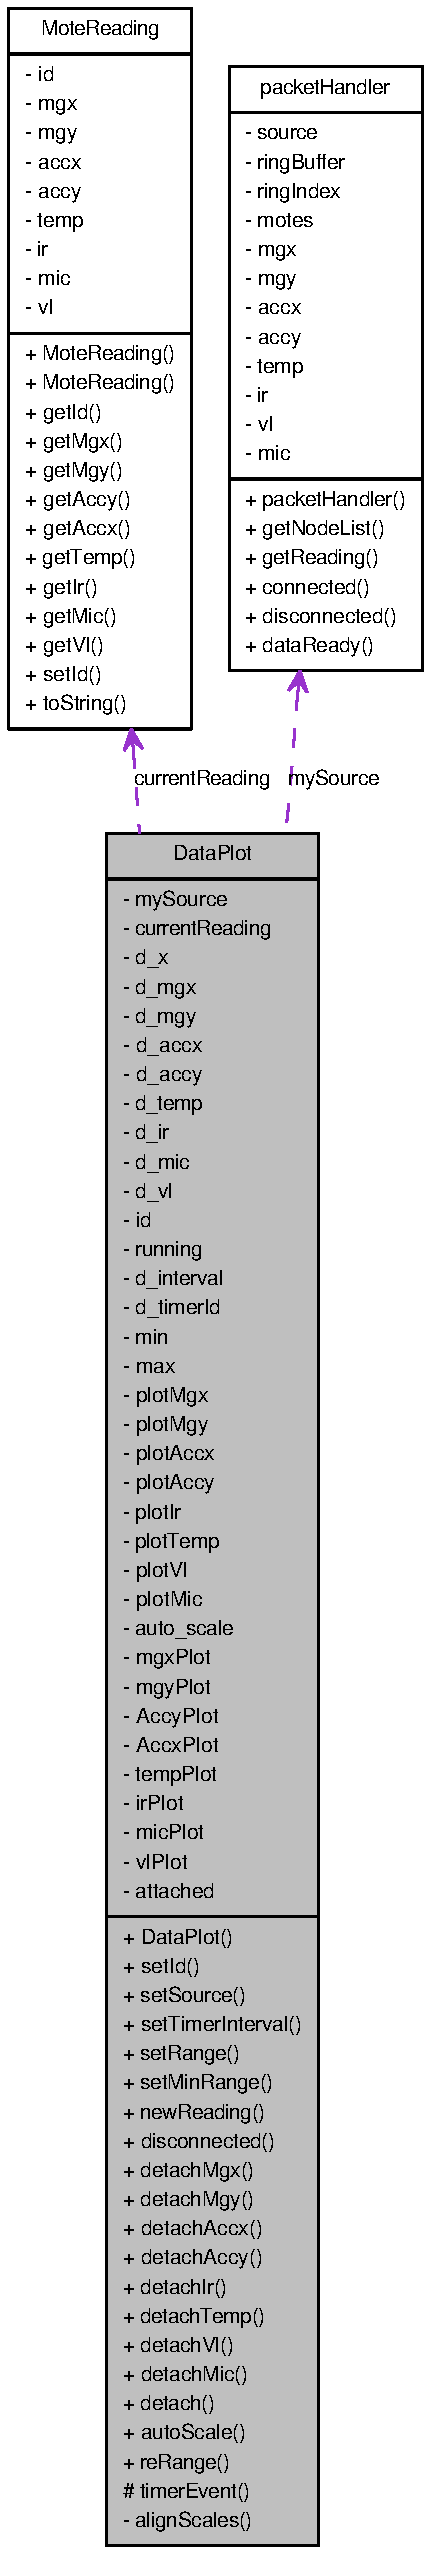
\includegraphics[height=400pt]{classDataPlot__coll__graph}
\end{center}
\end{figure}
\subsection*{Public Slots}
\begin{DoxyCompactItemize}
\item 
void \hyperlink{classDataPlot_a926020e0c49d78d3d5d282848368651e}{setTimerInterval} (double interval)
\item 
void \hyperlink{classDataPlot_a642185fdad89b1b075bc00670242fa0b}{setRange} (double range)
\item 
void \hyperlink{classDataPlot_ad101ac80563ee10322788946d791ea09}{setMinRange} (double range)
\item 
void \hyperlink{classDataPlot_a36fe7e25f67a168d4f7dd2eaa2627003}{newReading} (\hyperlink{classMoteReading}{MoteReading} r)
\item 
void \hyperlink{classDataPlot_a78920a414abdfa954fd34c662f39d09e}{disconnected} ()
\item 
void \hyperlink{classDataPlot_a74bc8f9c94caa90e092e1b3235c2c6ec}{detachMgx} ()
\item 
void \hyperlink{classDataPlot_a309a9e4dc84f977bc54f30d0e2cf2350}{detachMgy} ()
\item 
void \hyperlink{classDataPlot_a5dbafea843c682d18d77e1903e3c372b}{detachAccx} ()
\item 
void \hyperlink{classDataPlot_ab9a27391ec25592f1126f672716ab161}{detachAccy} ()
\item 
void \hyperlink{classDataPlot_a63ee85d95a1ce9b0ac889ea16c4827c7}{detachIr} ()
\item 
void \hyperlink{classDataPlot_a21893fd1f06b11e7e3286fa74e8c618f}{detachTemp} ()
\item 
void \hyperlink{classDataPlot_ad350cafabb24a175222744f7c7b3e10e}{detachVl} ()
\item 
void \hyperlink{classDataPlot_a42a2f46b248f64482153739201fc7d2b}{detachMic} ()
\item 
void \hyperlink{classDataPlot_a5521e1760646dbcf90df949e20523803}{detach} (int item)
\item 
void \hyperlink{classDataPlot_a6409fa9685624b4a453529254e6d943f}{autoScale} ()
\item 
void \hyperlink{classDataPlot_abc77f48da64170d587eda09e5aaf008c}{reRange} ()
\end{DoxyCompactItemize}
\subsection*{Public Member Functions}
\begin{DoxyCompactItemize}
\item 
\hyperlink{classDataPlot_a1343acbd6095212532c4315d6e9f1711}{DataPlot} (QWidget $\ast$=NULL)
\begin{DoxyCompactList}\small\item\em Default constructor. \item\end{DoxyCompactList}\item 
void \hyperlink{classDataPlot_ab6af06dfac3585a7dc669ea333a0869d}{setId} (int i)
\item 
void \hyperlink{classDataPlot_aace03b9e68e11042c0fade588e2869a7}{setSource} (\hyperlink{classpacketHandler}{packetHandler} $\ast$p)
\end{DoxyCompactItemize}
\subsection*{Protected Member Functions}
\begin{DoxyCompactItemize}
\item 
virtual void \hyperlink{classDataPlot_a41c9c4bc12d8d3e3abdf893c4fcfad7b}{timerEvent} (QTimerEvent $\ast$e)
\end{DoxyCompactItemize}


\subsection{Detailed Description}
The widget class that graphs the data. \begin{DoxyAuthor}{Author}
Jharrod LaFon 
\end{DoxyAuthor}
\begin{DoxyDate}{Date}
Spring 2010 
\end{DoxyDate}
\begin{DoxyRemark}{Remarks}
This class is used to plot data on a moving canvas. The data are acquired from an instance of the packet handler class. 
\end{DoxyRemark}


\subsection{Constructor \& Destructor Documentation}
\hypertarget{classDataPlot_a1343acbd6095212532c4315d6e9f1711}{
\index{DataPlot@{DataPlot}!DataPlot@{DataPlot}}
\index{DataPlot@{DataPlot}!DataPlot@{DataPlot}}
\subsubsection[{DataPlot}]{\setlength{\rightskip}{0pt plus 5cm}DataPlot::DataPlot (QWidget $\ast$ {\em parent} = {\ttfamily NULL})}}
\label{classDataPlot_a1343acbd6095212532c4315d6e9f1711}


Default constructor. 

Constructor.

Initializes the Main Window 

\begin{Desc}
\item[\hyperlink{todo__todo000001}{Todo}]Change line thickness \end{Desc}




Here is the call graph for this function:\nopagebreak
\begin{figure}[H]
\begin{center}
\leavevmode
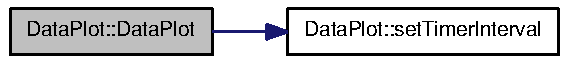
\includegraphics[width=154pt]{classDataPlot_a1343acbd6095212532c4315d6e9f1711_cgraph}
\end{center}
\end{figure}




\subsection{Member Function Documentation}
\hypertarget{classDataPlot_a6409fa9685624b4a453529254e6d943f}{
\index{DataPlot@{DataPlot}!autoScale@{autoScale}}
\index{autoScale@{autoScale}!DataPlot@{DataPlot}}
\subsubsection[{autoScale}]{\setlength{\rightskip}{0pt plus 5cm}void DataPlot::autoScale ()\hspace{0.3cm}{\ttfamily  \mbox{[}slot\mbox{]}}}}
\label{classDataPlot_a6409fa9685624b4a453529254e6d943f}
Enables or disables autoscaling \hypertarget{classDataPlot_a5521e1760646dbcf90df949e20523803}{
\index{DataPlot@{DataPlot}!detach@{detach}}
\index{detach@{detach}!DataPlot@{DataPlot}}
\subsubsection[{detach}]{\setlength{\rightskip}{0pt plus 5cm}void DataPlot::detach (int {\em item})\hspace{0.3cm}{\ttfamily  \mbox{[}slot\mbox{]}}}}
\label{classDataPlot_a5521e1760646dbcf90df949e20523803}
Slot for detaching a data type. 
\begin{DoxyParams}{Parameters}
\item[{\em item}]is from the enumeration defined in \hyperlink{data__plot_8h}{data\_\-plot.h} \end{DoxyParams}
\begin{DoxyNote}{Note}
This is actually a bad name. If the graph is already detached, it reattaches the graph. 
\end{DoxyNote}


Here is the caller graph for this function:\nopagebreak
\begin{figure}[H]
\begin{center}
\leavevmode
\includegraphics[width=142pt]{classDataPlot_a5521e1760646dbcf90df949e20523803_icgraph}
\end{center}
\end{figure}


\hypertarget{classDataPlot_a5dbafea843c682d18d77e1903e3c372b}{
\index{DataPlot@{DataPlot}!detachAccx@{detachAccx}}
\index{detachAccx@{detachAccx}!DataPlot@{DataPlot}}
\subsubsection[{detachAccx}]{\setlength{\rightskip}{0pt plus 5cm}void DataPlot::detachAccx ()\hspace{0.3cm}{\ttfamily  \mbox{[}inline, slot\mbox{]}}}}
\label{classDataPlot_a5dbafea843c682d18d77e1903e3c372b}
Slot for detaching ACCX 

Here is the call graph for this function:\nopagebreak
\begin{figure}[H]
\begin{center}
\leavevmode
\includegraphics[width=141pt]{classDataPlot_a5dbafea843c682d18d77e1903e3c372b_cgraph}
\end{center}
\end{figure}


\hypertarget{classDataPlot_ab9a27391ec25592f1126f672716ab161}{
\index{DataPlot@{DataPlot}!detachAccy@{detachAccy}}
\index{detachAccy@{detachAccy}!DataPlot@{DataPlot}}
\subsubsection[{detachAccy}]{\setlength{\rightskip}{0pt plus 5cm}void DataPlot::detachAccy ()\hspace{0.3cm}{\ttfamily  \mbox{[}inline, slot\mbox{]}}}}
\label{classDataPlot_ab9a27391ec25592f1126f672716ab161}
Slot for detaching ACCY 

Here is the call graph for this function:\nopagebreak
\begin{figure}[H]
\begin{center}
\leavevmode
\includegraphics[width=141pt]{classDataPlot_ab9a27391ec25592f1126f672716ab161_cgraph}
\end{center}
\end{figure}


\hypertarget{classDataPlot_a63ee85d95a1ce9b0ac889ea16c4827c7}{
\index{DataPlot@{DataPlot}!detachIr@{detachIr}}
\index{detachIr@{detachIr}!DataPlot@{DataPlot}}
\subsubsection[{detachIr}]{\setlength{\rightskip}{0pt plus 5cm}void DataPlot::detachIr ()\hspace{0.3cm}{\ttfamily  \mbox{[}inline, slot\mbox{]}}}}
\label{classDataPlot_a63ee85d95a1ce9b0ac889ea16c4827c7}
Slot for detaching IR 

Here is the call graph for this function:\nopagebreak
\begin{figure}[H]
\begin{center}
\leavevmode
\includegraphics[width=133pt]{classDataPlot_a63ee85d95a1ce9b0ac889ea16c4827c7_cgraph}
\end{center}
\end{figure}


\hypertarget{classDataPlot_a74bc8f9c94caa90e092e1b3235c2c6ec}{
\index{DataPlot@{DataPlot}!detachMgx@{detachMgx}}
\index{detachMgx@{detachMgx}!DataPlot@{DataPlot}}
\subsubsection[{detachMgx}]{\setlength{\rightskip}{0pt plus 5cm}void DataPlot::detachMgx ()\hspace{0.3cm}{\ttfamily  \mbox{[}inline, slot\mbox{]}}}}
\label{classDataPlot_a74bc8f9c94caa90e092e1b3235c2c6ec}
Slot for detaching MGx 

Here is the call graph for this function:\nopagebreak
\begin{figure}[H]
\begin{center}
\leavevmode
\includegraphics[width=139pt]{classDataPlot_a74bc8f9c94caa90e092e1b3235c2c6ec_cgraph}
\end{center}
\end{figure}


\hypertarget{classDataPlot_a309a9e4dc84f977bc54f30d0e2cf2350}{
\index{DataPlot@{DataPlot}!detachMgy@{detachMgy}}
\index{detachMgy@{detachMgy}!DataPlot@{DataPlot}}
\subsubsection[{detachMgy}]{\setlength{\rightskip}{0pt plus 5cm}void DataPlot::detachMgy ()\hspace{0.3cm}{\ttfamily  \mbox{[}inline, slot\mbox{]}}}}
\label{classDataPlot_a309a9e4dc84f977bc54f30d0e2cf2350}
Slot for detaching MGy 

Here is the call graph for this function:\nopagebreak
\begin{figure}[H]
\begin{center}
\leavevmode
\includegraphics[width=139pt]{classDataPlot_a309a9e4dc84f977bc54f30d0e2cf2350_cgraph}
\end{center}
\end{figure}


\hypertarget{classDataPlot_a42a2f46b248f64482153739201fc7d2b}{
\index{DataPlot@{DataPlot}!detachMic@{detachMic}}
\index{detachMic@{detachMic}!DataPlot@{DataPlot}}
\subsubsection[{detachMic}]{\setlength{\rightskip}{0pt plus 5cm}void DataPlot::detachMic ()\hspace{0.3cm}{\ttfamily  \mbox{[}inline, slot\mbox{]}}}}
\label{classDataPlot_a42a2f46b248f64482153739201fc7d2b}
Slot for detaching MIC 

Here is the call graph for this function:\nopagebreak
\begin{figure}[H]
\begin{center}
\leavevmode
\includegraphics[width=138pt]{classDataPlot_a42a2f46b248f64482153739201fc7d2b_cgraph}
\end{center}
\end{figure}


\hypertarget{classDataPlot_a21893fd1f06b11e7e3286fa74e8c618f}{
\index{DataPlot@{DataPlot}!detachTemp@{detachTemp}}
\index{detachTemp@{detachTemp}!DataPlot@{DataPlot}}
\subsubsection[{detachTemp}]{\setlength{\rightskip}{0pt plus 5cm}void DataPlot::detachTemp ()\hspace{0.3cm}{\ttfamily  \mbox{[}inline, slot\mbox{]}}}}
\label{classDataPlot_a21893fd1f06b11e7e3286fa74e8c618f}
Slot for detaching Temp 

Here is the call graph for this function:\nopagebreak
\begin{figure}[H]
\begin{center}
\leavevmode
\includegraphics[width=142pt]{classDataPlot_a21893fd1f06b11e7e3286fa74e8c618f_cgraph}
\end{center}
\end{figure}


\hypertarget{classDataPlot_ad350cafabb24a175222744f7c7b3e10e}{
\index{DataPlot@{DataPlot}!detachVl@{detachVl}}
\index{detachVl@{detachVl}!DataPlot@{DataPlot}}
\subsubsection[{detachVl}]{\setlength{\rightskip}{0pt plus 5cm}void DataPlot::detachVl ()\hspace{0.3cm}{\ttfamily  \mbox{[}inline, slot\mbox{]}}}}
\label{classDataPlot_ad350cafabb24a175222744f7c7b3e10e}
Slot for detaching VL 

Here is the call graph for this function:\nopagebreak
\begin{figure}[H]
\begin{center}
\leavevmode
\includegraphics[width=134pt]{classDataPlot_ad350cafabb24a175222744f7c7b3e10e_cgraph}
\end{center}
\end{figure}


\hypertarget{classDataPlot_a78920a414abdfa954fd34c662f39d09e}{
\index{DataPlot@{DataPlot}!disconnected@{disconnected}}
\index{disconnected@{disconnected}!DataPlot@{DataPlot}}
\subsubsection[{disconnected}]{\setlength{\rightskip}{0pt plus 5cm}void DataPlot::disconnected ()\hspace{0.3cm}{\ttfamily  \mbox{[}slot\mbox{]}}}}
\label{classDataPlot_a78920a414abdfa954fd34c662f39d09e}
Slot for notifying the datagraph that it's been disconnected from the packet source \hypertarget{classDataPlot_a36fe7e25f67a168d4f7dd2eaa2627003}{
\index{DataPlot@{DataPlot}!newReading@{newReading}}
\index{newReading@{newReading}!DataPlot@{DataPlot}}
\subsubsection[{newReading}]{\setlength{\rightskip}{0pt plus 5cm}void DataPlot::newReading ({\bf MoteReading} {\em r})\hspace{0.3cm}{\ttfamily  \mbox{[}slot\mbox{]}}}}
\label{classDataPlot_a36fe7e25f67a168d4f7dd2eaa2627003}
Slot for informing the graph of a new reading 
\begin{DoxyParams}{Parameters}
\item[{\em r}]The new mote reading \end{DoxyParams}


Here is the caller graph for this function:\nopagebreak
\begin{figure}[H]
\begin{center}
\leavevmode
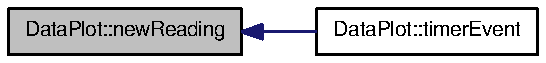
\includegraphics[width=149pt]{classDataPlot_a36fe7e25f67a168d4f7dd2eaa2627003_icgraph}
\end{center}
\end{figure}


\hypertarget{classDataPlot_abc77f48da64170d587eda09e5aaf008c}{
\index{DataPlot@{DataPlot}!reRange@{reRange}}
\index{reRange@{reRange}!DataPlot@{DataPlot}}
\subsubsection[{reRange}]{\setlength{\rightskip}{0pt plus 5cm}void DataPlot::reRange ()\hspace{0.3cm}{\ttfamily  \mbox{[}slot\mbox{]}}}}
\label{classDataPlot_abc77f48da64170d587eda09e5aaf008c}
Resets the viewing window of the graph 

Here is the caller graph for this function:\nopagebreak
\begin{figure}[H]
\begin{center}
\leavevmode
\includegraphics[width=141pt]{classDataPlot_abc77f48da64170d587eda09e5aaf008c_icgraph}
\end{center}
\end{figure}


\hypertarget{classDataPlot_ab6af06dfac3585a7dc669ea333a0869d}{
\index{DataPlot@{DataPlot}!setId@{setId}}
\index{setId@{setId}!DataPlot@{DataPlot}}
\subsubsection[{setId}]{\setlength{\rightskip}{0pt plus 5cm}void DataPlot::setId (int {\em i})\hspace{0.3cm}{\ttfamily  \mbox{[}inline\mbox{]}}}}
\label{classDataPlot_ab6af06dfac3585a7dc669ea333a0869d}
Sets the dataGraph's id. Used to demultiplex mote readings. 
\begin{DoxyParams}{Parameters}
\item[{\em i}]\end{DoxyParams}
\begin{DoxyReturn}{Returns}
void 
\end{DoxyReturn}
\hypertarget{classDataPlot_ad101ac80563ee10322788946d791ea09}{
\index{DataPlot@{DataPlot}!setMinRange@{setMinRange}}
\index{setMinRange@{setMinRange}!DataPlot@{DataPlot}}
\subsubsection[{setMinRange}]{\setlength{\rightskip}{0pt plus 5cm}void DataPlot::setMinRange (double {\em range})\hspace{0.3cm}{\ttfamily  \mbox{[}slot\mbox{]}}}}
\label{classDataPlot_ad101ac80563ee10322788946d791ea09}
Slot for setting the lower range of the graph 
\begin{DoxyParams}{Parameters}
\item[{\em range}]is the lower bound of the viewing window \end{DoxyParams}


\begin{DoxyNote}{Note}
Old Bug: Qt Doesn't capture this event for some reason. Fixed this bug. 
\end{DoxyNote}


\hypertarget{classDataPlot_a642185fdad89b1b075bc00670242fa0b}{
\index{DataPlot@{DataPlot}!setRange@{setRange}}
\index{setRange@{setRange}!DataPlot@{DataPlot}}
\subsubsection[{setRange}]{\setlength{\rightskip}{0pt plus 5cm}void DataPlot::setRange (double {\em range})\hspace{0.3cm}{\ttfamily  \mbox{[}slot\mbox{]}}}}
\label{classDataPlot_a642185fdad89b1b075bc00670242fa0b}
Slot for setting the upper range of the graph 
\begin{DoxyParams}{Parameters}
\item[{\em range}]The upper bound of the viewing window \end{DoxyParams}
\hypertarget{classDataPlot_aace03b9e68e11042c0fade588e2869a7}{
\index{DataPlot@{DataPlot}!setSource@{setSource}}
\index{setSource@{setSource}!DataPlot@{DataPlot}}
\subsubsection[{setSource}]{\setlength{\rightskip}{0pt plus 5cm}void DataPlot::setSource ({\bf packetHandler} $\ast$ {\em p})\hspace{0.3cm}{\ttfamily  \mbox{[}inline\mbox{]}}}}
\label{classDataPlot_aace03b9e68e11042c0fade588e2869a7}
Mutator for packetHander Use this to set the \hyperlink{classpacketHandler}{packetHandler} (server) for this plot 
\begin{DoxyParams}{Parameters}
\item[{\em p}]Pointer to the \hyperlink{classpacketHandler}{packetHandler} \end{DoxyParams}


Here is the caller graph for this function:\nopagebreak
\begin{figure}[H]
\begin{center}
\leavevmode
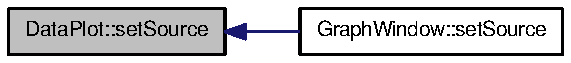
\includegraphics[width=155pt]{classDataPlot_aace03b9e68e11042c0fade588e2869a7_icgraph}
\end{center}
\end{figure}


\hypertarget{classDataPlot_a926020e0c49d78d3d5d282848368651e}{
\index{DataPlot@{DataPlot}!setTimerInterval@{setTimerInterval}}
\index{setTimerInterval@{setTimerInterval}!DataPlot@{DataPlot}}
\subsubsection[{setTimerInterval}]{\setlength{\rightskip}{0pt plus 5cm}void DataPlot::setTimerInterval (double {\em interval})\hspace{0.3cm}{\ttfamily  \mbox{[}slot\mbox{]}}}}
\label{classDataPlot_a926020e0c49d78d3d5d282848368651e}
Slot for changing the timer frequency 
\begin{DoxyParams}{Parameters}
\item[{\em interval}]The frequency of sampling \end{DoxyParams}


\begin{DoxyRemark}{Remarks}
Units are in ms 
\end{DoxyRemark}




Here is the caller graph for this function:\nopagebreak
\begin{figure}[H]
\begin{center}
\leavevmode
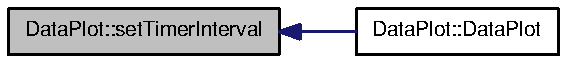
\includegraphics[width=154pt]{classDataPlot_a926020e0c49d78d3d5d282848368651e_icgraph}
\end{center}
\end{figure}


\hypertarget{classDataPlot_a41c9c4bc12d8d3e3abdf893c4fcfad7b}{
\index{DataPlot@{DataPlot}!timerEvent@{timerEvent}}
\index{timerEvent@{timerEvent}!DataPlot@{DataPlot}}
\subsubsection[{timerEvent}]{\setlength{\rightskip}{0pt plus 5cm}void DataPlot::timerEvent (QTimerEvent $\ast$ {\em e})\hspace{0.3cm}{\ttfamily  \mbox{[}protected, virtual\mbox{]}}}}
\label{classDataPlot_a41c9c4bc12d8d3e3abdf893c4fcfad7b}
Timer event function

\begin{DoxyRemark}{Remarks}
This gets called to update the graph. 
\end{DoxyRemark}


\begin{Desc}
\item[\hyperlink{todo__todo000002}{Todo}]Make this scale more intelligently. \end{Desc}




Here is the call graph for this function:\nopagebreak
\begin{figure}[H]
\begin{center}
\leavevmode
\includegraphics[width=160pt]{classDataPlot_a41c9c4bc12d8d3e3abdf893c4fcfad7b_cgraph}
\end{center}
\end{figure}




The documentation for this class was generated from the following files:\begin{DoxyCompactItemize}
\item 
\hyperlink{data__plot_8h}{data\_\-plot.h}\item 
\hyperlink{data__plot_8cpp}{data\_\-plot.cpp}\end{DoxyCompactItemize}

\hypertarget{classGraphWindow}{
\section{GraphWindow Class Reference}
\label{classGraphWindow}\index{GraphWindow@{GraphWindow}}
}


Window class that contains the \hyperlink{classDataPlot}{DataPlot} widget.  




{\ttfamily \#include $<$graphwindow.h$>$}



Collaboration diagram for GraphWindow:\nopagebreak
\begin{figure}[H]
\begin{center}
\leavevmode
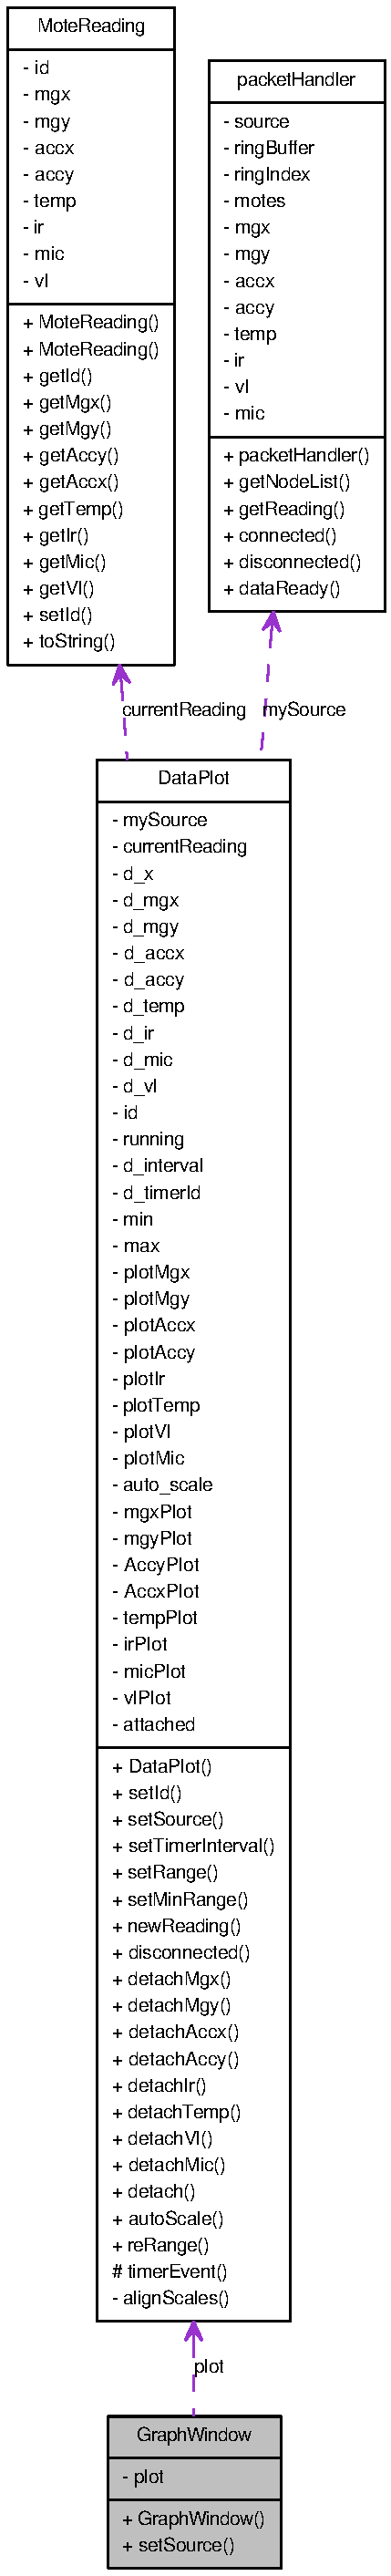
\includegraphics[height=400pt]{classGraphWindow__coll__graph}
\end{center}
\end{figure}
\subsection*{Public Member Functions}
\begin{DoxyCompactItemize}
\item 
\hypertarget{classGraphWindow_ab8ca84cf6fe5a68e7fb87b7f47636d7d}{
\hyperlink{classGraphWindow_ab8ca84cf6fe5a68e7fb87b7f47636d7d}{GraphWindow} ()}
\label{classGraphWindow_ab8ca84cf6fe5a68e7fb87b7f47636d7d}

\begin{DoxyCompactList}\small\item\em Default constructor. \item\end{DoxyCompactList}\item 
void \hyperlink{classGraphWindow_a07a46e21184c287ba49db8145047e420}{setSource} (\hyperlink{classpacketHandler}{packetHandler} $\ast$p)
\begin{DoxyCompactList}\small\item\em Sets the data source. \item\end{DoxyCompactList}\end{DoxyCompactItemize}


\subsection{Detailed Description}
Window class that contains the \hyperlink{classDataPlot}{DataPlot} widget. \begin{DoxyAuthor}{Author}
Jharrod LaFon 
\end{DoxyAuthor}
\begin{DoxyDate}{Date}
Spring 2010 
\end{DoxyDate}


\subsection{Member Function Documentation}
\hypertarget{classGraphWindow_a07a46e21184c287ba49db8145047e420}{
\index{GraphWindow@{GraphWindow}!setSource@{setSource}}
\index{setSource@{setSource}!GraphWindow@{GraphWindow}}
\subsubsection[{setSource}]{\setlength{\rightskip}{0pt plus 5cm}void GraphWindow::setSource ({\bf packetHandler} $\ast$ {\em p})}}
\label{classGraphWindow_a07a46e21184c287ba49db8145047e420}


Sets the data source. 

\begin{DoxyRemark}{Remarks}
This also sets the source for the dataplot class. 
\end{DoxyRemark}


Here is the call graph for this function:\nopagebreak
\begin{figure}[H]
\begin{center}
\leavevmode
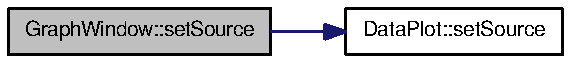
\includegraphics[width=155pt]{classGraphWindow_a07a46e21184c287ba49db8145047e420_cgraph}
\end{center}
\end{figure}




The documentation for this class was generated from the following files:\begin{DoxyCompactItemize}
\item 
\hyperlink{graphwindow_8h}{graphwindow.h}\item 
\hyperlink{graphwindow_8cpp}{graphwindow.cpp}\end{DoxyCompactItemize}

\hypertarget{classMainWindow}{
\section{MainWindow Class Reference}
\label{classMainWindow}\index{MainWindow@{MainWindow}}
}


The main window class.  




{\ttfamily \#include $<$mainwindow.h$>$}



Collaboration diagram for MainWindow:\nopagebreak
\begin{figure}[H]
\begin{center}
\leavevmode
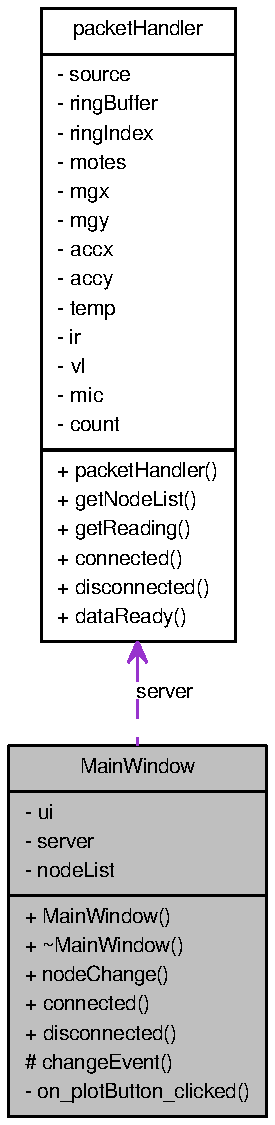
\includegraphics[height=400pt]{classMainWindow__coll__graph}
\end{center}
\end{figure}
\subsection*{Public Slots}
\begin{DoxyCompactItemize}
\item 
\hypertarget{classMainWindow_a5d0ce13b14ee5fe76a4f7ed7f1de81c5}{
void \hyperlink{classMainWindow_a5d0ce13b14ee5fe76a4f7ed7f1de81c5}{nodeChange} ()}
\label{classMainWindow_a5d0ce13b14ee5fe76a4f7ed7f1de81c5}

\begin{DoxyCompactList}\small\item\em Updates the nodeList widget when a node is added or removed from the packet stream. \item\end{DoxyCompactList}\end{DoxyCompactItemize}
\subsection*{Public Member Functions}
\begin{DoxyCompactItemize}
\item 
\hypertarget{classMainWindow_a8b244be8b7b7db1b08de2a2acb9409db}{
\hyperlink{classMainWindow_a8b244be8b7b7db1b08de2a2acb9409db}{MainWindow} (QWidget $\ast$parent=0)}
\label{classMainWindow_a8b244be8b7b7db1b08de2a2acb9409db}

\begin{DoxyCompactList}\small\item\em Default constructor. \item\end{DoxyCompactList}\item 
\hypertarget{classMainWindow_ae98d00a93bc118200eeef9f9bba1dba7}{
\hyperlink{classMainWindow_ae98d00a93bc118200eeef9f9bba1dba7}{$\sim$MainWindow} ()}
\label{classMainWindow_ae98d00a93bc118200eeef9f9bba1dba7}

\begin{DoxyCompactList}\small\item\em Destructor. \item\end{DoxyCompactList}\end{DoxyCompactItemize}
\subsection*{Protected Member Functions}
\begin{DoxyCompactItemize}
\item 
\hypertarget{classMainWindow_af4ca5d0d3d18ddcb7d54b6596bbf4797}{
void \hyperlink{classMainWindow_af4ca5d0d3d18ddcb7d54b6596bbf4797}{changeEvent} (QEvent $\ast$e)}
\label{classMainWindow_af4ca5d0d3d18ddcb7d54b6596bbf4797}

\begin{DoxyCompactList}\small\item\em Needed for Qt. \item\end{DoxyCompactList}\end{DoxyCompactItemize}


\subsection{Detailed Description}
The main window class. \begin{DoxyAuthor}{Author}
Jharrod LaFon 
\end{DoxyAuthor}
\begin{DoxyDate}{Date}
Spring 2010 
\end{DoxyDate}
\begin{DoxyRemark}{Remarks}
Main Window class. Inherits from QMainWindow 
\end{DoxyRemark}


The documentation for this class was generated from the following files:\begin{DoxyCompactItemize}
\item 
\hyperlink{mainwindow_8h}{mainwindow.h}\item 
\hyperlink{mainwindow_8cpp}{mainwindow.cpp}\end{DoxyCompactItemize}

\hypertarget{classMoteReading}{
\section{MoteReading Class Reference}
\label{classMoteReading}\index{MoteReading@{MoteReading}}
}


Class to encapsulate a sensor reading.  




{\ttfamily \#include $<$motereading.h$>$}

\subsection*{Public Member Functions}
\begin{DoxyCompactItemize}
\item 
\hyperlink{classMoteReading_ad2555254ab4fd4ce31ebafeea362d255}{MoteReading} ()
\begin{DoxyCompactList}\small\item\em Default constructor. \item\end{DoxyCompactList}\item 
\hyperlink{classMoteReading_aea4d9a40d3999ed29eb6044146a5dabc}{MoteReading} (int id, int mgx, int mgy, int accx, int accy, int temp, int ir, int mic, int vl)
\item 
int \hyperlink{classMoteReading_a123a08348d6a1ba80a4055cb5f5afaa6}{getId} ()
\begin{DoxyCompactList}\small\item\em Accessor for id. \item\end{DoxyCompactList}\item 
int \hyperlink{classMoteReading_a318b7e6afba062ee3df207495070e277}{getMgx} ()
\begin{DoxyCompactList}\small\item\em Accessor for magnetometer x. \item\end{DoxyCompactList}\item 
int \hyperlink{classMoteReading_a4344f67449dbd79febac0c4795b185f4}{getMgy} ()
\begin{DoxyCompactList}\small\item\em Accessor for magnetometer y. \item\end{DoxyCompactList}\item 
int \hyperlink{classMoteReading_af918c7ca6c9fea98a3d608b61dbaffae}{getAccy} ()
\begin{DoxyCompactList}\small\item\em Accessor for accelerometer y. \item\end{DoxyCompactList}\item 
int \hyperlink{classMoteReading_ad79a65f84dfaacc9b5c179fb66a5545f}{getAccx} ()
\begin{DoxyCompactList}\small\item\em Accessor for acclerometer x. \item\end{DoxyCompactList}\item 
int \hyperlink{classMoteReading_a3f7526c29f2bf61feeb5e24298133332}{getTemp} ()
\begin{DoxyCompactList}\small\item\em Accessor for temperature. \item\end{DoxyCompactList}\item 
int \hyperlink{classMoteReading_aff0d87f9c667d01f7e37a114afa321fa}{getIr} ()
\begin{DoxyCompactList}\small\item\em Accessor for infrared. \item\end{DoxyCompactList}\item 
int \hyperlink{classMoteReading_a348cb45f4613499385a354fe6857ef5d}{getMic} ()
\begin{DoxyCompactList}\small\item\em Accessor for microphone. \item\end{DoxyCompactList}\item 
int \hyperlink{classMoteReading_a88ed6ea245c7af79e38ff8976f849f36}{getVl} ()
\begin{DoxyCompactList}\small\item\em Accessor for visual light. \item\end{DoxyCompactList}\item 
void \hyperlink{classMoteReading_a61f08f015a9f833ff7352c378b7799c2}{setId} (int i)
\begin{DoxyCompactList}\small\item\em Mutator for id. \item\end{DoxyCompactList}\item 
QString \hyperlink{classMoteReading_a5e60715c001c14f3e3f4cff6f886f0ad}{toString} ()
\begin{DoxyCompactList}\small\item\em Accessor for string representation of reading. \item\end{DoxyCompactList}\end{DoxyCompactItemize}


\subsection{Detailed Description}
Class to encapsulate a sensor reading. \begin{DoxyAuthor}{Author}
Jharrod LaFon 
\end{DoxyAuthor}
\begin{DoxyDate}{Date}
Spring 2010 
\end{DoxyDate}
\begin{DoxyRemark}{Remarks}
Class to encapsulate mote readings. 
\end{DoxyRemark}


Definition at line 15 of file motereading.h.



\subsection{Constructor \& Destructor Documentation}
\hypertarget{classMoteReading_ad2555254ab4fd4ce31ebafeea362d255}{
\index{MoteReading@{MoteReading}!MoteReading@{MoteReading}}
\index{MoteReading@{MoteReading}!MoteReading@{MoteReading}}
\subsubsection[{MoteReading}]{\setlength{\rightskip}{0pt plus 5cm}MoteReading::MoteReading ()}}
\label{classMoteReading_ad2555254ab4fd4ce31ebafeea362d255}


Default constructor. 

\begin{Desc}
\item[\hyperlink{todo__todo000003}{Todo}]Create copy constructor \end{Desc}


Definition at line 10 of file motereading.cpp.




\begin{DoxyCode}
11 {
12 
13 }
\end{DoxyCode}


\hypertarget{classMoteReading_aea4d9a40d3999ed29eb6044146a5dabc}{
\index{MoteReading@{MoteReading}!MoteReading@{MoteReading}}
\index{MoteReading@{MoteReading}!MoteReading@{MoteReading}}
\subsubsection[{MoteReading}]{\setlength{\rightskip}{0pt plus 5cm}MoteReading::MoteReading (int {\em id}, \/  int {\em mgx}, \/  int {\em mgy}, \/  int {\em accx}, \/  int {\em accy}, \/  int {\em temp}, \/  int {\em ir}, \/  int {\em mic}, \/  int {\em vl})}}
\label{classMoteReading_aea4d9a40d3999ed29eb6044146a5dabc}
Constructor, takes all readings as parameters 
\begin{DoxyParams}{Parameters}
\item[{\em id,mgx,mgy,accx,accy,temp,ir,mic,vl}]\end{DoxyParams}


Definition at line 16 of file motereading.cpp.




\begin{DoxyCode}
17  {
18 
19      id = m_id;
20      mgx = m_mgx;
21      mgy = m_mgy;
22      accx = m_accx;
23      accy = m_accy;
24      temp = m_temp;
25      ir = m_ir;
26      mic = m_mic;
27      vl = m_vl;
28  }
\end{DoxyCode}




\subsection{Member Function Documentation}
\hypertarget{classMoteReading_ad79a65f84dfaacc9b5c179fb66a5545f}{
\index{MoteReading@{MoteReading}!getAccx@{getAccx}}
\index{getAccx@{getAccx}!MoteReading@{MoteReading}}
\subsubsection[{getAccx}]{\setlength{\rightskip}{0pt plus 5cm}int MoteReading::getAccx ()\hspace{0.3cm}{\ttfamily  \mbox{[}inline\mbox{]}}}}
\label{classMoteReading_ad79a65f84dfaacc9b5c179fb66a5545f}


Accessor for acclerometer x. 

\begin{DoxyReturn}{Returns}
accx 
\end{DoxyReturn}


Definition at line 48 of file motereading.h.




\begin{DoxyCode}
48 { return accx; }
\end{DoxyCode}




Here is the caller graph for this function:\nopagebreak
\begin{figure}[H]
\begin{center}
\leavevmode
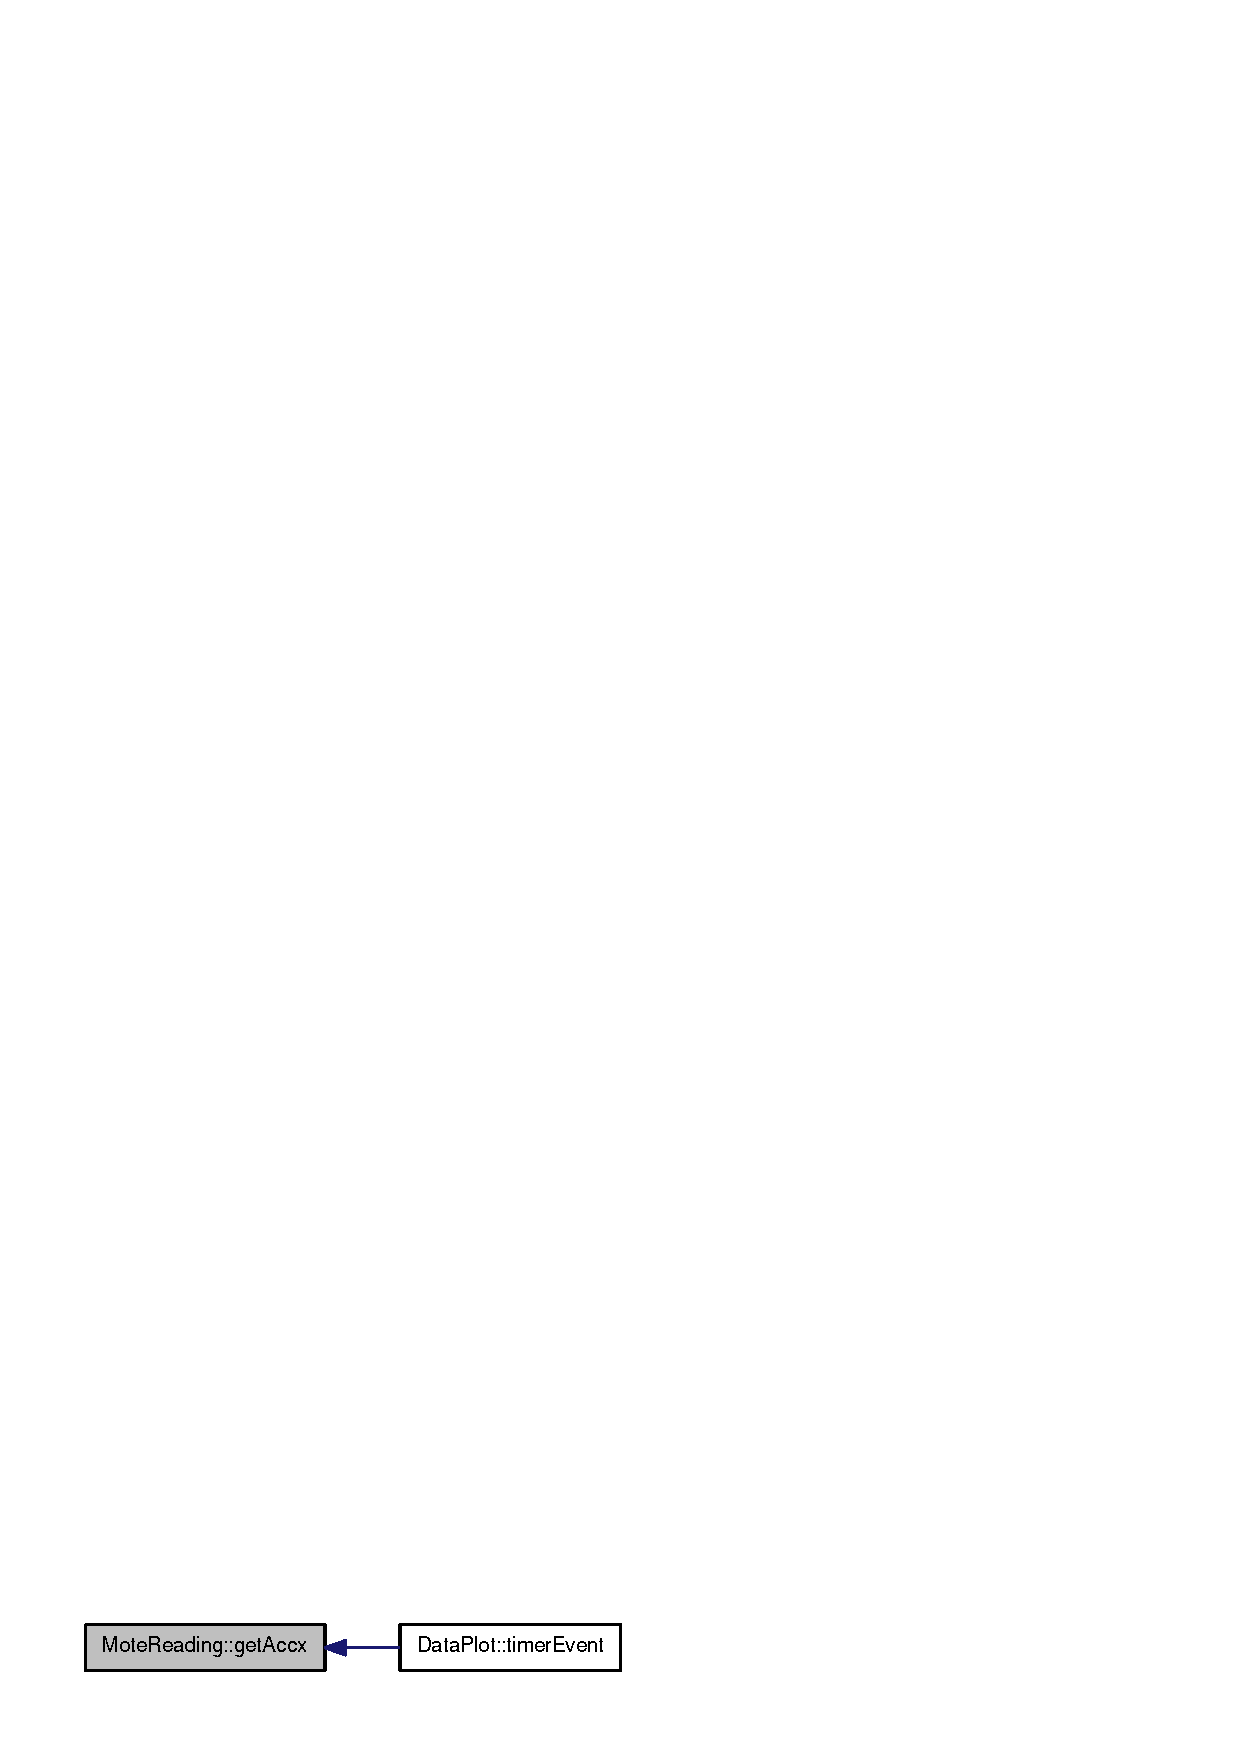
\includegraphics[width=151pt]{classMoteReading_ad79a65f84dfaacc9b5c179fb66a5545f_icgraph}
\end{center}
\end{figure}


\hypertarget{classMoteReading_af918c7ca6c9fea98a3d608b61dbaffae}{
\index{MoteReading@{MoteReading}!getAccy@{getAccy}}
\index{getAccy@{getAccy}!MoteReading@{MoteReading}}
\subsubsection[{getAccy}]{\setlength{\rightskip}{0pt plus 5cm}int MoteReading::getAccy ()\hspace{0.3cm}{\ttfamily  \mbox{[}inline\mbox{]}}}}
\label{classMoteReading_af918c7ca6c9fea98a3d608b61dbaffae}


Accessor for accelerometer y. 

\begin{DoxyReturn}{Returns}
mgy 
\end{DoxyReturn}


Definition at line 43 of file motereading.h.




\begin{DoxyCode}
43 { return accy; }
\end{DoxyCode}




Here is the caller graph for this function:\nopagebreak
\begin{figure}[H]
\begin{center}
\leavevmode
\includegraphics[width=151pt]{classMoteReading_af918c7ca6c9fea98a3d608b61dbaffae_icgraph}
\end{center}
\end{figure}


\hypertarget{classMoteReading_a123a08348d6a1ba80a4055cb5f5afaa6}{
\index{MoteReading@{MoteReading}!getId@{getId}}
\index{getId@{getId}!MoteReading@{MoteReading}}
\subsubsection[{getId}]{\setlength{\rightskip}{0pt plus 5cm}int MoteReading::getId ()\hspace{0.3cm}{\ttfamily  \mbox{[}inline\mbox{]}}}}
\label{classMoteReading_a123a08348d6a1ba80a4055cb5f5afaa6}


Accessor for id. 

\begin{DoxyReturn}{Returns}
id 
\end{DoxyReturn}


Definition at line 28 of file motereading.h.




\begin{DoxyCode}
28 { return id; }
\end{DoxyCode}


\hypertarget{classMoteReading_aff0d87f9c667d01f7e37a114afa321fa}{
\index{MoteReading@{MoteReading}!getIr@{getIr}}
\index{getIr@{getIr}!MoteReading@{MoteReading}}
\subsubsection[{getIr}]{\setlength{\rightskip}{0pt plus 5cm}int MoteReading::getIr ()\hspace{0.3cm}{\ttfamily  \mbox{[}inline\mbox{]}}}}
\label{classMoteReading_aff0d87f9c667d01f7e37a114afa321fa}


Accessor for infrared. 

\begin{DoxyReturn}{Returns}
ir 
\end{DoxyReturn}


Definition at line 58 of file motereading.h.




\begin{DoxyCode}
58 { return ir; }
\end{DoxyCode}




Here is the caller graph for this function:\nopagebreak
\begin{figure}[H]
\begin{center}
\leavevmode
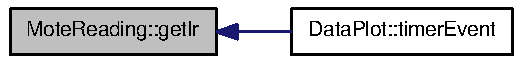
\includegraphics[width=143pt]{classMoteReading_aff0d87f9c667d01f7e37a114afa321fa_icgraph}
\end{center}
\end{figure}


\hypertarget{classMoteReading_a318b7e6afba062ee3df207495070e277}{
\index{MoteReading@{MoteReading}!getMgx@{getMgx}}
\index{getMgx@{getMgx}!MoteReading@{MoteReading}}
\subsubsection[{getMgx}]{\setlength{\rightskip}{0pt plus 5cm}int MoteReading::getMgx ()\hspace{0.3cm}{\ttfamily  \mbox{[}inline\mbox{]}}}}
\label{classMoteReading_a318b7e6afba062ee3df207495070e277}


Accessor for magnetometer x. 

\begin{DoxyReturn}{Returns}
mgx 
\end{DoxyReturn}


Definition at line 33 of file motereading.h.




\begin{DoxyCode}
33 { return mgx; }
\end{DoxyCode}




Here is the caller graph for this function:\nopagebreak
\begin{figure}[H]
\begin{center}
\leavevmode
\includegraphics[width=149pt]{classMoteReading_a318b7e6afba062ee3df207495070e277_icgraph}
\end{center}
\end{figure}


\hypertarget{classMoteReading_a4344f67449dbd79febac0c4795b185f4}{
\index{MoteReading@{MoteReading}!getMgy@{getMgy}}
\index{getMgy@{getMgy}!MoteReading@{MoteReading}}
\subsubsection[{getMgy}]{\setlength{\rightskip}{0pt plus 5cm}int MoteReading::getMgy ()\hspace{0.3cm}{\ttfamily  \mbox{[}inline\mbox{]}}}}
\label{classMoteReading_a4344f67449dbd79febac0c4795b185f4}


Accessor for magnetometer y. 

\begin{DoxyReturn}{Returns}
mgy 
\end{DoxyReturn}


Definition at line 38 of file motereading.h.




\begin{DoxyCode}
38 { return mgy; }
\end{DoxyCode}




Here is the caller graph for this function:\nopagebreak
\begin{figure}[H]
\begin{center}
\leavevmode
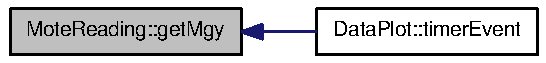
\includegraphics[width=149pt]{classMoteReading_a4344f67449dbd79febac0c4795b185f4_icgraph}
\end{center}
\end{figure}


\hypertarget{classMoteReading_a348cb45f4613499385a354fe6857ef5d}{
\index{MoteReading@{MoteReading}!getMic@{getMic}}
\index{getMic@{getMic}!MoteReading@{MoteReading}}
\subsubsection[{getMic}]{\setlength{\rightskip}{0pt plus 5cm}int MoteReading::getMic ()\hspace{0.3cm}{\ttfamily  \mbox{[}inline\mbox{]}}}}
\label{classMoteReading_a348cb45f4613499385a354fe6857ef5d}


Accessor for microphone. 

\begin{DoxyReturn}{Returns}
mic 
\end{DoxyReturn}


Definition at line 63 of file motereading.h.




\begin{DoxyCode}
63 { return mic; }
\end{DoxyCode}




Here is the caller graph for this function:\nopagebreak
\begin{figure}[H]
\begin{center}
\leavevmode
\includegraphics[width=147pt]{classMoteReading_a348cb45f4613499385a354fe6857ef5d_icgraph}
\end{center}
\end{figure}


\hypertarget{classMoteReading_a3f7526c29f2bf61feeb5e24298133332}{
\index{MoteReading@{MoteReading}!getTemp@{getTemp}}
\index{getTemp@{getTemp}!MoteReading@{MoteReading}}
\subsubsection[{getTemp}]{\setlength{\rightskip}{0pt plus 5cm}int MoteReading::getTemp ()\hspace{0.3cm}{\ttfamily  \mbox{[}inline\mbox{]}}}}
\label{classMoteReading_a3f7526c29f2bf61feeb5e24298133332}


Accessor for temperature. 

\begin{DoxyReturn}{Returns}
temp 
\end{DoxyReturn}


Definition at line 53 of file motereading.h.




\begin{DoxyCode}
53 { return temp; }
\end{DoxyCode}




Here is the caller graph for this function:\nopagebreak
\begin{figure}[H]
\begin{center}
\leavevmode
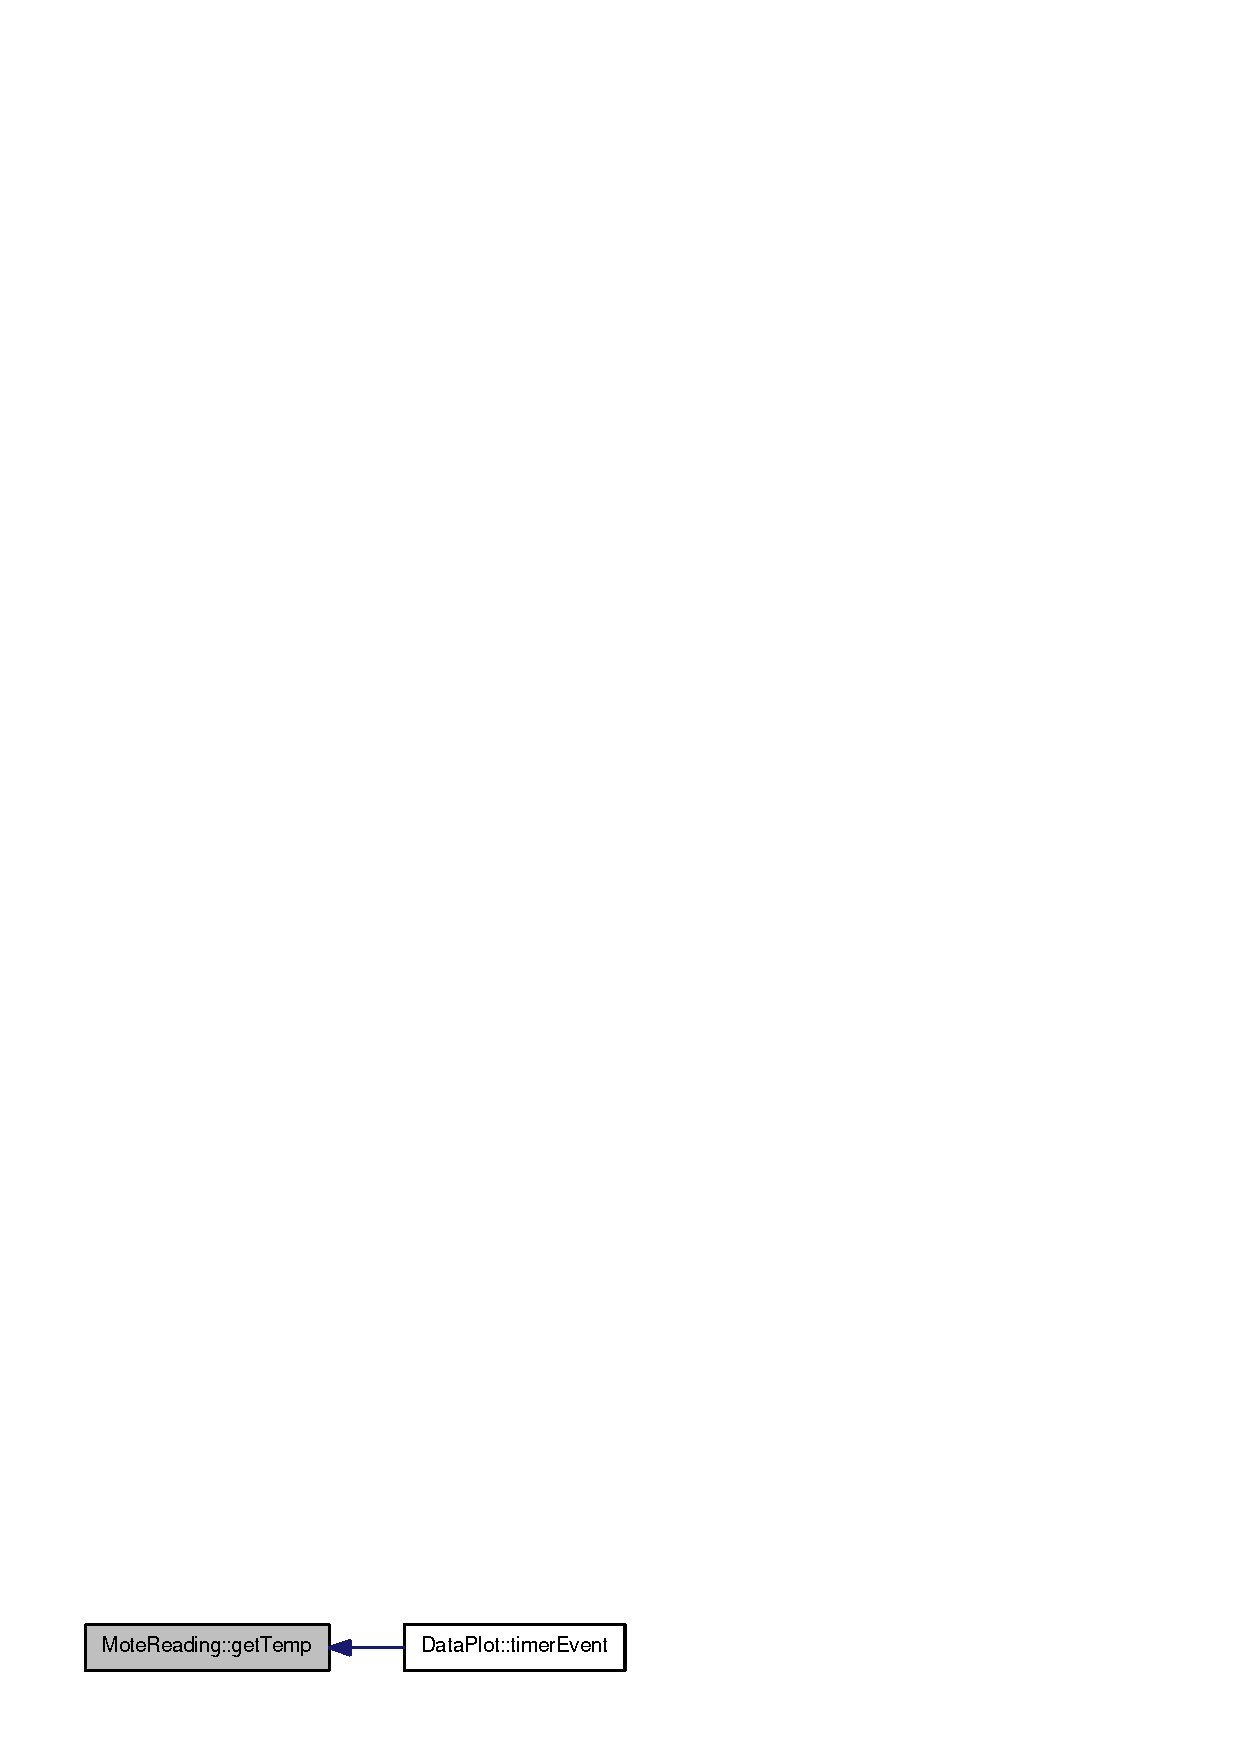
\includegraphics[width=152pt]{classMoteReading_a3f7526c29f2bf61feeb5e24298133332_icgraph}
\end{center}
\end{figure}


\hypertarget{classMoteReading_a88ed6ea245c7af79e38ff8976f849f36}{
\index{MoteReading@{MoteReading}!getVl@{getVl}}
\index{getVl@{getVl}!MoteReading@{MoteReading}}
\subsubsection[{getVl}]{\setlength{\rightskip}{0pt plus 5cm}int MoteReading::getVl ()\hspace{0.3cm}{\ttfamily  \mbox{[}inline\mbox{]}}}}
\label{classMoteReading_a88ed6ea245c7af79e38ff8976f849f36}


Accessor for visual light. 

\begin{DoxyReturn}{Returns}
int visual\_\-light 
\end{DoxyReturn}


Definition at line 68 of file motereading.h.




\begin{DoxyCode}
68 { return vl; }
\end{DoxyCode}




Here is the caller graph for this function:\nopagebreak
\begin{figure}[H]
\begin{center}
\leavevmode
\includegraphics[width=144pt]{classMoteReading_a88ed6ea245c7af79e38ff8976f849f36_icgraph}
\end{center}
\end{figure}


\hypertarget{classMoteReading_a61f08f015a9f833ff7352c378b7799c2}{
\index{MoteReading@{MoteReading}!setId@{setId}}
\index{setId@{setId}!MoteReading@{MoteReading}}
\subsubsection[{setId}]{\setlength{\rightskip}{0pt plus 5cm}void MoteReading::setId (int {\em i})\hspace{0.3cm}{\ttfamily  \mbox{[}inline\mbox{]}}}}
\label{classMoteReading_a61f08f015a9f833ff7352c378b7799c2}


Mutator for id. 


\begin{DoxyParams}{Parameters}
\item[{\em i}]\end{DoxyParams}


Definition at line 73 of file motereading.h.




\begin{DoxyCode}
73 { id = i; }
\end{DoxyCode}


\hypertarget{classMoteReading_a5e60715c001c14f3e3f4cff6f886f0ad}{
\index{MoteReading@{MoteReading}!toString@{toString}}
\index{toString@{toString}!MoteReading@{MoteReading}}
\subsubsection[{toString}]{\setlength{\rightskip}{0pt plus 5cm}QString MoteReading::toString ()\hspace{0.3cm}{\ttfamily  \mbox{[}inline\mbox{]}}}}
\label{classMoteReading_a5e60715c001c14f3e3f4cff6f886f0ad}


Accessor for string representation of reading. 

\begin{DoxyReturn}{Returns}
QString 
\end{DoxyReturn}


Definition at line 78 of file motereading.h.




\begin{DoxyCode}
78 { return QString("%1 %2 %2 %4 %5 %6 %7 %8").arg(mgx).arg(mgy).arg(accx).arg(accy)
      .arg(temp).arg(ir).arg(mic).arg(vl); }
\end{DoxyCode}




The documentation for this class was generated from the following files:\begin{DoxyCompactItemize}
\item 
\hyperlink{motereading_8h}{motereading.h}\item 
\hyperlink{motereading_8cpp}{motereading.cpp}\end{DoxyCompactItemize}

\hypertarget{classpacketHandler}{
\section{packetHandler Class Reference}
\label{classpacketHandler}\index{packetHandler@{packetHandler}}
}


Class the serve packets to the \hyperlink{classDataPlot}{DataPlot}.  




{\ttfamily \#include $<$packethandler.h$>$}

\subsection*{Public Slots}
\begin{DoxyCompactItemize}
\item 
\hypertarget{classpacketHandler_ab1a61d0c1deef1885e31b9a6aebdcc2f}{
void \hyperlink{classpacketHandler_ab1a61d0c1deef1885e31b9a6aebdcc2f}{connected} ()}
\label{classpacketHandler_ab1a61d0c1deef1885e31b9a6aebdcc2f}

\begin{DoxyCompactList}\small\item\em Slot for when a connection is established. This also initializes communication with the serial forwarder. \item\end{DoxyCompactList}\item 
void \hyperlink{classpacketHandler_a43223a8930a6af8c40c5889d8e4b9d4b}{disconnected} ()
\begin{DoxyCompactList}\small\item\em Slot for when we are disconnected from the serial forwarder. \item\end{DoxyCompactList}\item 
void \hyperlink{classpacketHandler_a9085a61a51eccc7acb240a7b68601686}{dataReady} ()
\begin{DoxyCompactList}\small\item\em Slot for when there is new data ready from the serial forwarder. \item\end{DoxyCompactList}\end{DoxyCompactItemize}
\subsection*{Signals}
\begin{DoxyCompactItemize}
\item 
\hypertarget{classpacketHandler_a0e8f4d081f531b5e568c052f5b8babb9}{
void \hyperlink{classpacketHandler_a0e8f4d081f531b5e568c052f5b8babb9}{nodesChanged} ()}
\label{classpacketHandler_a0e8f4d081f531b5e568c052f5b8babb9}

\begin{DoxyCompactList}\small\item\em Signal emitted when a new node is detected. \item\end{DoxyCompactList}\item 
\hypertarget{classpacketHandler_a033895b001ec68791c5d0872df03e626}{
void \hyperlink{classpacketHandler_a033895b001ec68791c5d0872df03e626}{disconnectNotice} ()}
\label{classpacketHandler_a033895b001ec68791c5d0872df03e626}

\begin{DoxyCompactList}\small\item\em Signal emitted when disconnected from the serial forwarder. \item\end{DoxyCompactList}\end{DoxyCompactItemize}
\subsection*{Public Member Functions}
\begin{DoxyCompactItemize}
\item 
\hyperlink{classpacketHandler_a02936b9105618ed38701274efcfa0dfb}{packetHandler} ()
\begin{DoxyCompactList}\small\item\em Default constructor. \item\end{DoxyCompactList}\item 
QList$<$ int $>$ \hyperlink{classpacketHandler_a7d07166d577b014234ad311599ac3291}{getNodeList} ()
\item 
\hyperlink{classMoteReading}{MoteReading} \hyperlink{classpacketHandler_aec6fa94602daa18227491b76001152cb}{getReading} (int i)
\end{DoxyCompactItemize}


\subsection{Detailed Description}
Class the serve packets to the \hyperlink{classDataPlot}{DataPlot}. \begin{DoxyAuthor}{Author}
Jharrod LaFon 
\end{DoxyAuthor}
\begin{DoxyDate}{Date}
Spring 2010 
\end{DoxyDate}
\begin{DoxyRemark}{Remarks}
This class connects to the serial forwarder, and demultiplexes packets for the datagraph class. 
\end{DoxyRemark}


\subsection{Constructor \& Destructor Documentation}
\hypertarget{classpacketHandler_a02936b9105618ed38701274efcfa0dfb}{
\index{packetHandler@{packetHandler}!packetHandler@{packetHandler}}
\index{packetHandler@{packetHandler}!packetHandler@{packetHandler}}
\subsubsection[{packetHandler}]{\setlength{\rightskip}{0pt plus 5cm}packetHandler::packetHandler ()}}
\label{classpacketHandler_a02936b9105618ed38701274efcfa0dfb}


Default constructor. 



\begin{Desc}
\item[\hyperlink{todo__todo000004}{Todo}]Make this connection user configurable. \end{Desc}




Here is the call graph for this function:\nopagebreak
\begin{figure}[H]
\begin{center}
\leavevmode
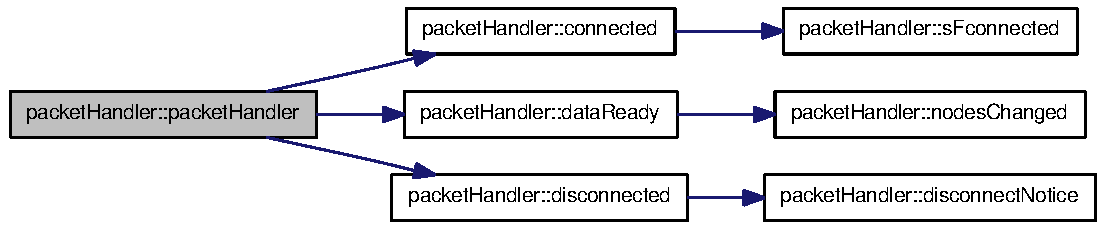
\includegraphics[width=283pt]{classpacketHandler_a02936b9105618ed38701274efcfa0dfb_cgraph}
\end{center}
\end{figure}




\subsection{Member Function Documentation}
\hypertarget{classpacketHandler_a9085a61a51eccc7acb240a7b68601686}{
\index{packetHandler@{packetHandler}!dataReady@{dataReady}}
\index{dataReady@{dataReady}!packetHandler@{packetHandler}}
\subsubsection[{dataReady}]{\setlength{\rightskip}{0pt plus 5cm}void packetHandler::dataReady ()\hspace{0.3cm}{\ttfamily  \mbox{[}slot\mbox{]}}}}
\label{classpacketHandler_a9085a61a51eccc7acb240a7b68601686}


Slot for when there is new data ready from the serial forwarder. 



\begin{DoxyRemark}{Remarks}
Up to MAX\_\-BUFFER packets are stored in a ringBuffer for each mote. 
\end{DoxyRemark}




Here is the call graph for this function:\nopagebreak
\begin{figure}[H]
\begin{center}
\leavevmode
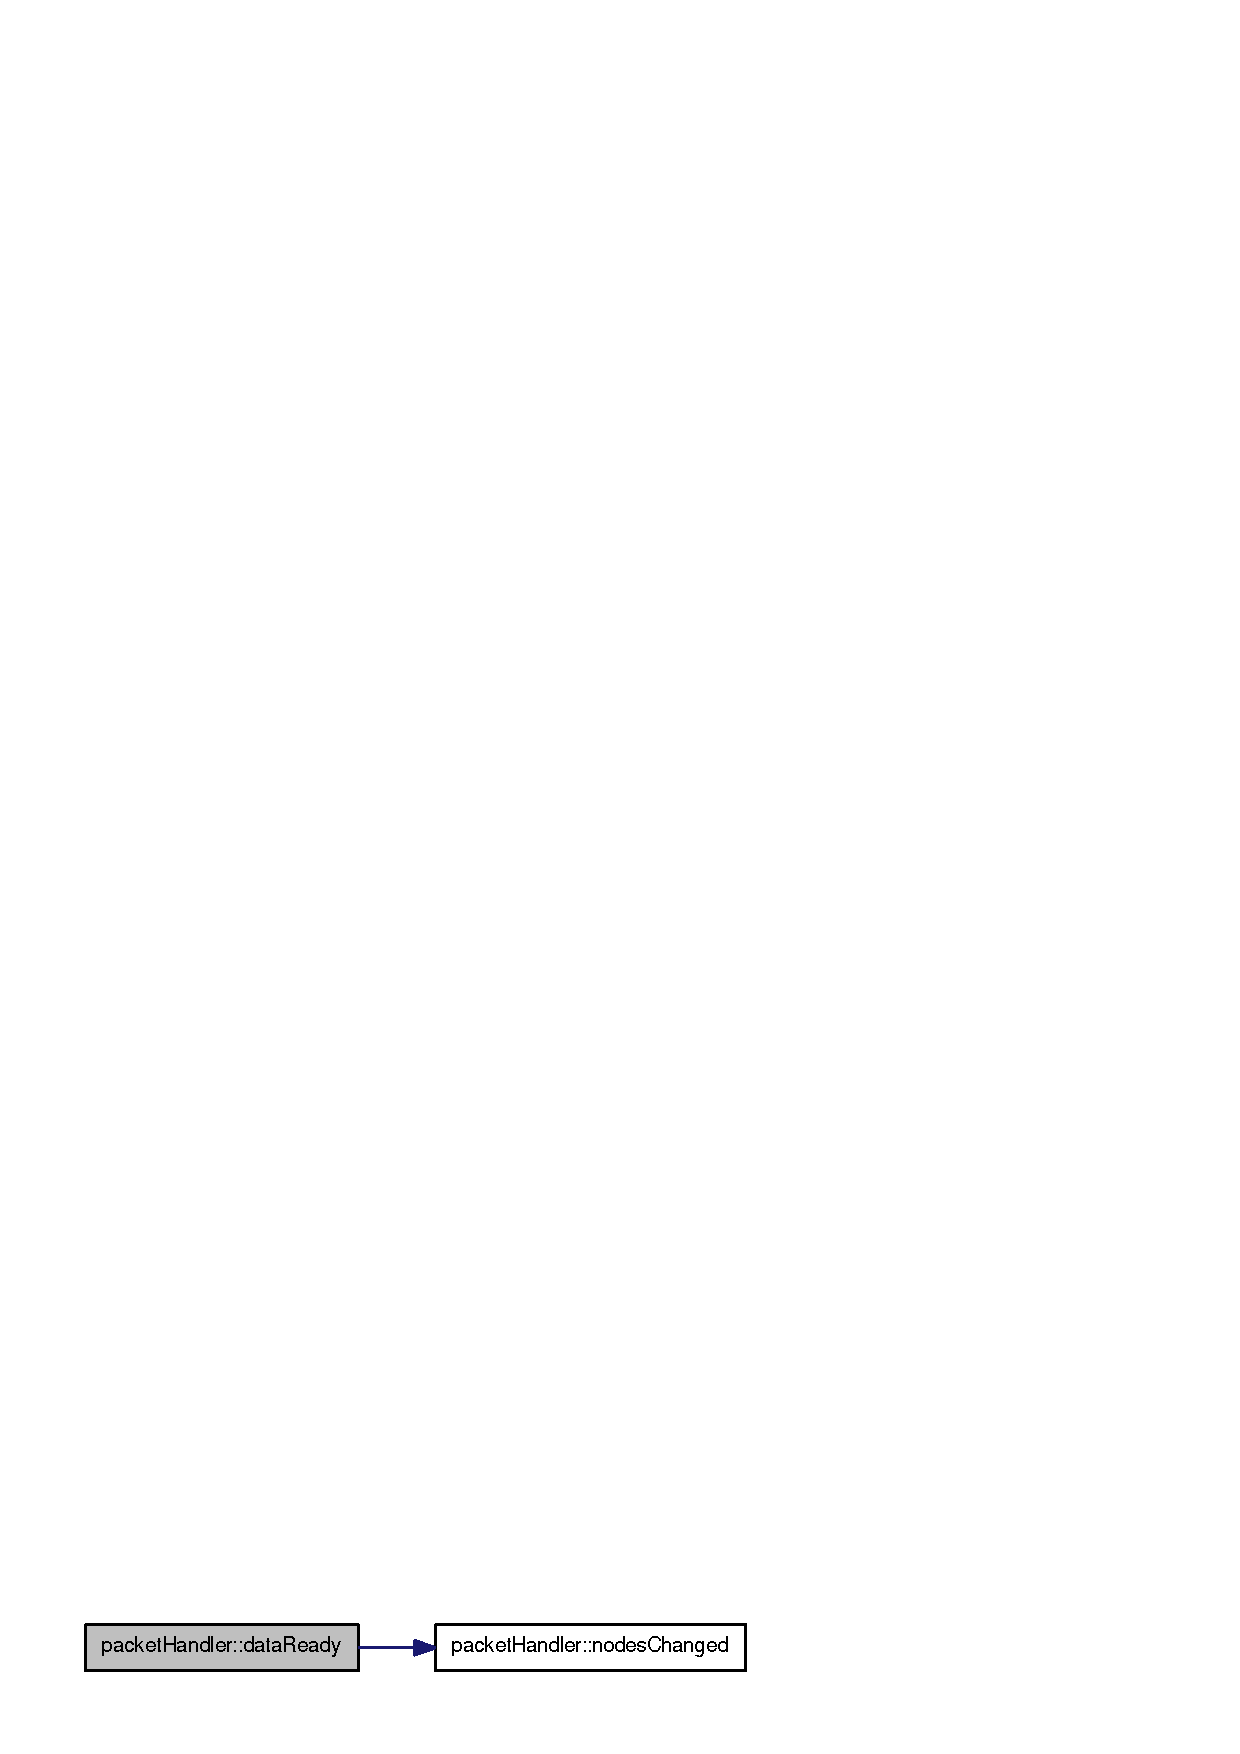
\includegraphics[width=181pt]{classpacketHandler_a9085a61a51eccc7acb240a7b68601686_cgraph}
\end{center}
\end{figure}




Here is the caller graph for this function:\nopagebreak
\begin{figure}[H]
\begin{center}
\leavevmode
\includegraphics[width=180pt]{classpacketHandler_a9085a61a51eccc7acb240a7b68601686_icgraph}
\end{center}
\end{figure}


\hypertarget{classpacketHandler_a43223a8930a6af8c40c5889d8e4b9d4b}{
\index{packetHandler@{packetHandler}!disconnected@{disconnected}}
\index{disconnected@{disconnected}!packetHandler@{packetHandler}}
\subsubsection[{disconnected}]{\setlength{\rightskip}{0pt plus 5cm}void packetHandler::disconnected ()\hspace{0.3cm}{\ttfamily  \mbox{[}slot\mbox{]}}}}
\label{classpacketHandler_a43223a8930a6af8c40c5889d8e4b9d4b}


Slot for when we are disconnected from the serial forwarder. 

\begin{DoxyRemark}{Remarks}
This gets called when the TcpSocket is disconnected, so we tell the dataGraph class also. 
\end{DoxyRemark}


Here is the call graph for this function:\nopagebreak
\begin{figure}[H]
\begin{center}
\leavevmode
\includegraphics[width=191pt]{classpacketHandler_a43223a8930a6af8c40c5889d8e4b9d4b_cgraph}
\end{center}
\end{figure}




Here is the caller graph for this function:\nopagebreak
\begin{figure}[H]
\begin{center}
\leavevmode
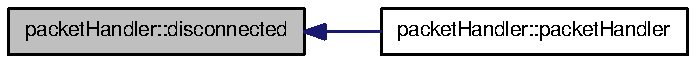
\includegraphics[width=185pt]{classpacketHandler_a43223a8930a6af8c40c5889d8e4b9d4b_icgraph}
\end{center}
\end{figure}


\hypertarget{classpacketHandler_a7d07166d577b014234ad311599ac3291}{
\index{packetHandler@{packetHandler}!getNodeList@{getNodeList}}
\index{getNodeList@{getNodeList}!packetHandler@{packetHandler}}
\subsubsection[{getNodeList}]{\setlength{\rightskip}{0pt plus 5cm}QList$<$ int $>$ packetHandler::getNodeList ()}}
\label{classpacketHandler_a7d07166d577b014234ad311599ac3291}
Function to return the list of nodes from which we have received packets. \begin{DoxyReturn}{Returns}
QList$<$int$>$ 
\end{DoxyReturn}


Here is the caller graph for this function:\nopagebreak
\begin{figure}[H]
\begin{center}
\leavevmode
\includegraphics[width=258pt]{classpacketHandler_a7d07166d577b014234ad311599ac3291_icgraph}
\end{center}
\end{figure}


\hypertarget{classpacketHandler_aec6fa94602daa18227491b76001152cb}{
\index{packetHandler@{packetHandler}!getReading@{getReading}}
\index{getReading@{getReading}!packetHandler@{packetHandler}}
\subsubsection[{getReading}]{\setlength{\rightskip}{0pt plus 5cm}{\bf MoteReading} packetHandler::getReading (int {\em i})}}
\label{classpacketHandler_aec6fa94602daa18227491b76001152cb}
Function to get the most recent reading for node i 
\begin{DoxyParams}{Parameters}
\item[{\em i}]The id of the mote. \end{DoxyParams}
\begin{DoxyReturn}{Returns}
\hyperlink{classMoteReading}{MoteReading} 
\end{DoxyReturn}


\begin{Desc}
\item[\hyperlink{bug__bug000002}{Bug}]I need to get this working correctly, but I'm not sure on the logic yet. \end{Desc}




Here is the caller graph for this function:\nopagebreak
\begin{figure}[H]
\begin{center}
\leavevmode
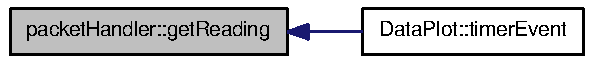
\includegraphics[width=160pt]{classpacketHandler_aec6fa94602daa18227491b76001152cb_icgraph}
\end{center}
\end{figure}




The documentation for this class was generated from the following files:\begin{DoxyCompactItemize}
\item 
\hyperlink{packethandler_8h}{packethandler.h}\item 
\hyperlink{packethandler_8cpp}{packethandler.cpp}\end{DoxyCompactItemize}

\chapter{File Documentation}
\hypertarget{data__plot_8cpp}{
\section{data\_\-plot.cpp File Reference}
\label{data__plot_8cpp}\index{data\_\-plot.cpp@{data\_\-plot.cpp}}
}


Implementation of \hyperlink{classDataPlot}{DataPlot} class.  


{\ttfamily \#include $<$QDebug$>$}\par
{\ttfamily \#include $<$qwt\_\-painter.h$>$}\par
{\ttfamily \#include $<$qwt\_\-plot\_\-canvas.h$>$}\par
{\ttfamily \#include $<$qwt\_\-plot\_\-marker.h$>$}\par
{\ttfamily \#include $<$qwt\_\-plot\_\-curve.h$>$}\par
{\ttfamily \#include $<$qwt\_\-scale\_\-widget.h$>$}\par
{\ttfamily \#include $<$qwt\_\-legend.h$>$}\par
{\ttfamily \#include $<$qwt\_\-scale\_\-draw.h$>$}\par
{\ttfamily \#include $<$qwt\_\-math.h$>$}\par
{\ttfamily \#include \char`\"{}data\_\-plot.h\char`\"{}}\par
{\ttfamily \#include $<$qwt\_\-plot.h$>$}\par
{\ttfamily \#include $<$QTcpSocket$>$}\par
{\ttfamily \#include $<$QList$>$}\par
{\ttfamily \#include $<$QObject$>$}\par
{\ttfamily \#include $<$QString$>$}\par
{\ttfamily \#include \char`\"{}motereading.h\char`\"{}}\par
{\ttfamily \#include \char`\"{}packethandler.h\char`\"{}}\par
Include dependency graph for data\_\-plot.cpp:\nopagebreak
\begin{figure}[H]
\begin{center}
\leavevmode
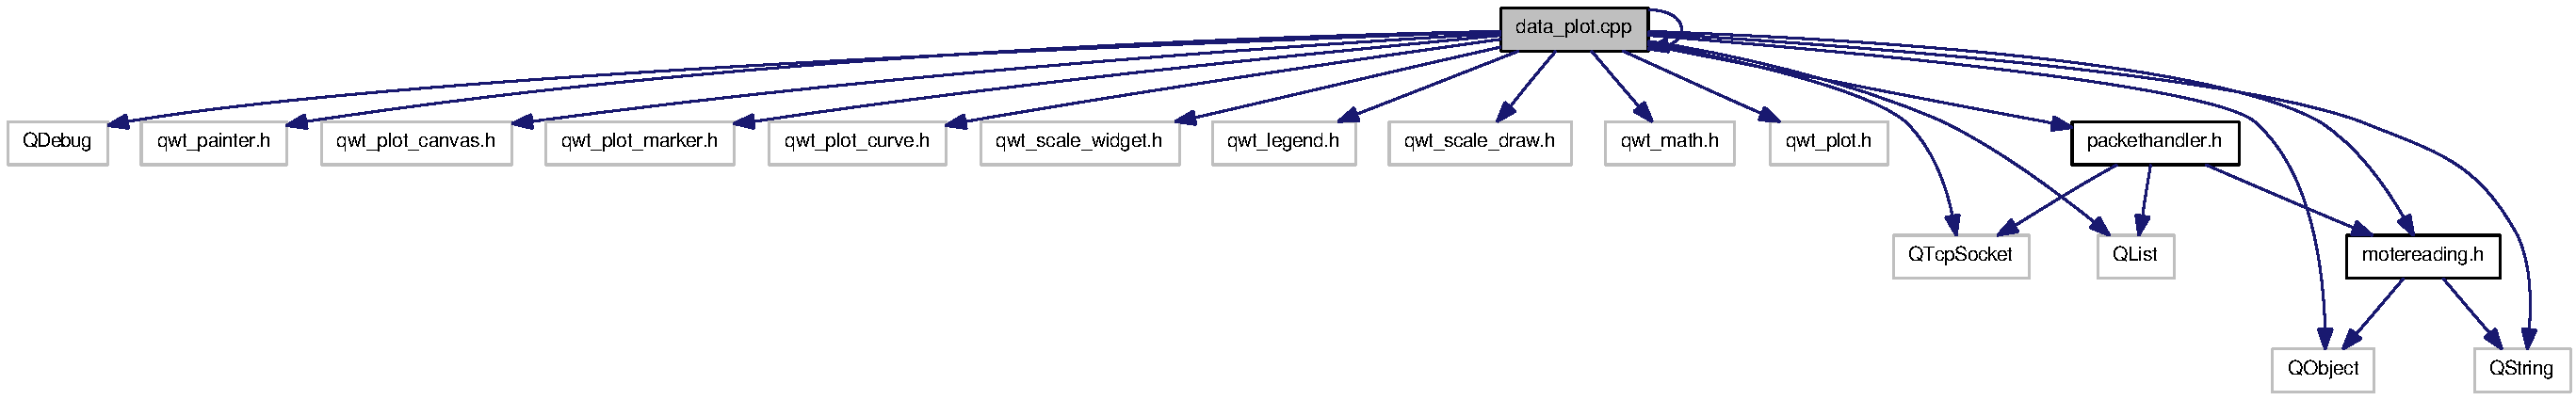
\includegraphics[width=420pt]{data__plot_8cpp__incl}
\end{center}
\end{figure}
This graph shows which files directly or indirectly include this file:\nopagebreak
\begin{figure}[H]
\begin{center}
\leavevmode
\includegraphics[width=68pt]{data__plot_8cpp__dep__incl}
\end{center}
\end{figure}


\subsection{Detailed Description}
Implementation of \hyperlink{classDataPlot}{DataPlot} class. \begin{DoxyAuthor}{Author}
Jharrod LaFon 
\end{DoxyAuthor}
\begin{DoxyDate}{Date}
Spring 2010 
\end{DoxyDate}

\hypertarget{data__plot_8h}{
\section{data\_\-plot.h File Reference}
\label{data__plot_8h}\index{data\_\-plot.h@{data\_\-plot.h}}
}


Widget to graph data.  


{\ttfamily \#include $<$qwt\_\-plot.h$>$}\par
{\ttfamily \#include $<$QDebug$>$}\par
{\ttfamily \#include $<$qwt\_\-painter.h$>$}\par
{\ttfamily \#include $<$qwt\_\-plot\_\-canvas.h$>$}\par
{\ttfamily \#include $<$qwt\_\-plot\_\-marker.h$>$}\par
{\ttfamily \#include $<$qwt\_\-plot\_\-curve.h$>$}\par
{\ttfamily \#include $<$qwt\_\-scale\_\-widget.h$>$}\par
{\ttfamily \#include $<$qwt\_\-legend.h$>$}\par
{\ttfamily \#include $<$qwt\_\-scale\_\-draw.h$>$}\par
{\ttfamily \#include $<$qwt\_\-math.h$>$}\par
{\ttfamily \#include \char`\"{}packethandler.h\char`\"{}}\par
{\ttfamily \#include \char`\"{}motereading.h\char`\"{}}\par
Include dependency graph for data\_\-plot.h:\nopagebreak
\begin{figure}[H]
\begin{center}
\leavevmode
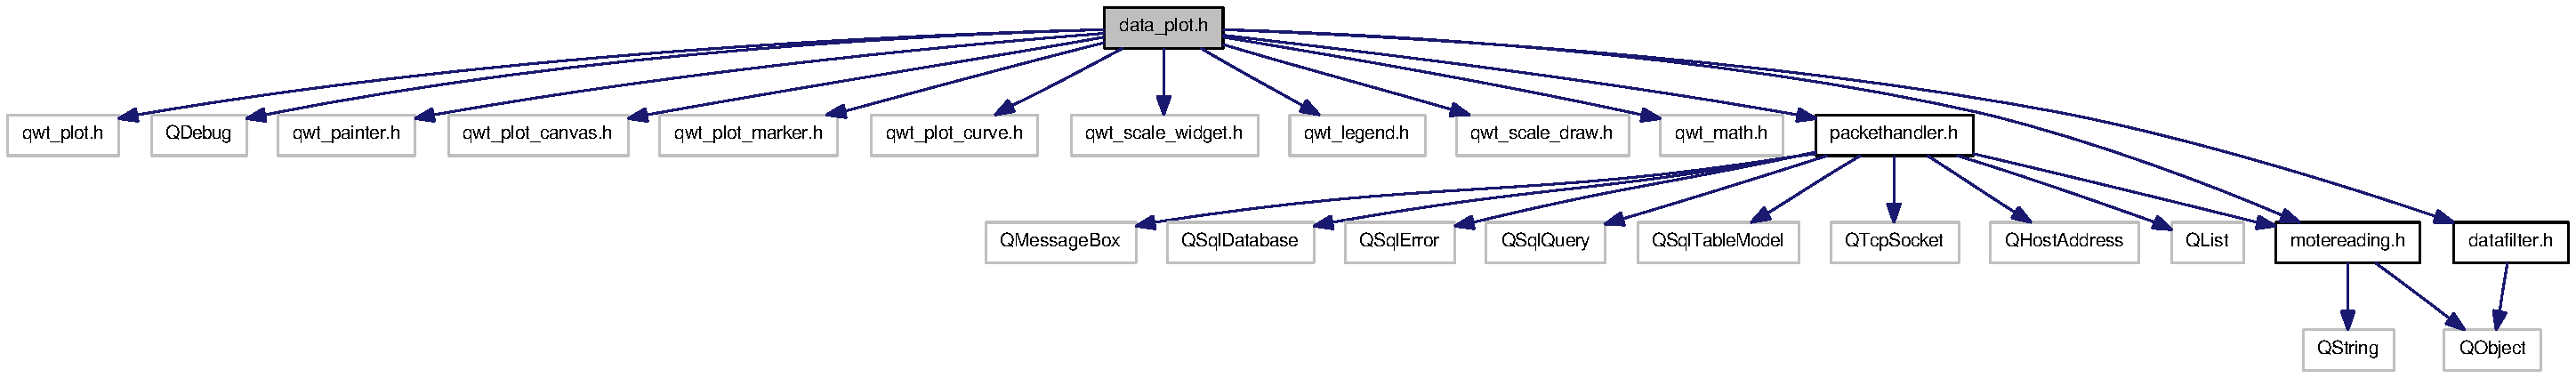
\includegraphics[width=420pt]{data__plot_8h__incl}
\end{center}
\end{figure}
This graph shows which files directly or indirectly include this file:\nopagebreak
\begin{figure}[H]
\begin{center}
\leavevmode
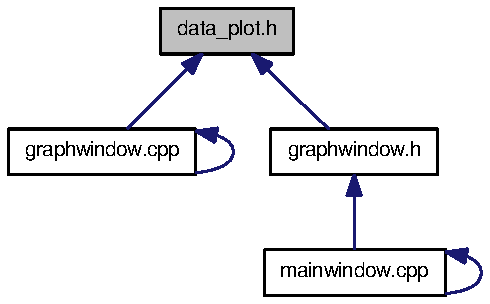
\includegraphics[width=135pt]{data__plot_8h__dep__incl}
\end{center}
\end{figure}
\subsection*{Classes}
\begin{DoxyCompactItemize}
\item 
class \hyperlink{classDataPlot}{DataPlot}
\begin{DoxyCompactList}\small\item\em The widget class that graphs the data. \item\end{DoxyCompactList}\end{DoxyCompactItemize}
\subsection*{Enumerations}
\begin{DoxyCompactItemize}
\item 
enum \{ \par
{\bfseries MGX}, 
{\bfseries MGY}, 
{\bfseries ACCX}, 
{\bfseries ACCY}, 
\par
{\bfseries IR}, 
{\bfseries TEMP}, 
{\bfseries VL}, 
{\bfseries MIC}
 \}
\end{DoxyCompactItemize}
\subsection*{Variables}
\begin{DoxyCompactItemize}
\item 
\hypertarget{data__plot_8h_aa335ff27182dcf42a50b762e32d8c184}{
const int \hyperlink{data__plot_8h_aa335ff27182dcf42a50b762e32d8c184}{PLOT\_\-SIZE} = 201}
\label{data__plot_8h_aa335ff27182dcf42a50b762e32d8c184}

\begin{DoxyCompactList}\small\item\em Size of the plot. \item\end{DoxyCompactList}\end{DoxyCompactItemize}


\subsection{Detailed Description}
Widget to graph data. 

Definition in file \hyperlink{data__plot_8h_source}{data\_\-plot.h}.


\hypertarget{graphwindow_8cpp}{
\section{graphwindow.cpp File Reference}
\label{graphwindow_8cpp}\index{graphwindow.cpp@{graphwindow.cpp}}
}


Implementation of the \hyperlink{classGraphWindow}{GraphWindow} class.  


{\ttfamily \#include \char`\"{}graphwindow.h\char`\"{}}\par
{\ttfamily \#include $<$qmainwindow.h$>$}\par
{\ttfamily \#include \char`\"{}data\_\-plot.h\char`\"{}}\par
{\ttfamily \#include $<$qwt\_\-counter.h$>$}\par
{\ttfamily \#include $<$qtoolbar.h$>$}\par
{\ttfamily \#include $<$qlabel.h$>$}\par
{\ttfamily \#include $<$qlayout.h$>$}\par
{\ttfamily \#include \char`\"{}packethandler.h\char`\"{}}\par
Include dependency graph for graphwindow.cpp:\nopagebreak
\begin{figure}[H]
\begin{center}
\leavevmode
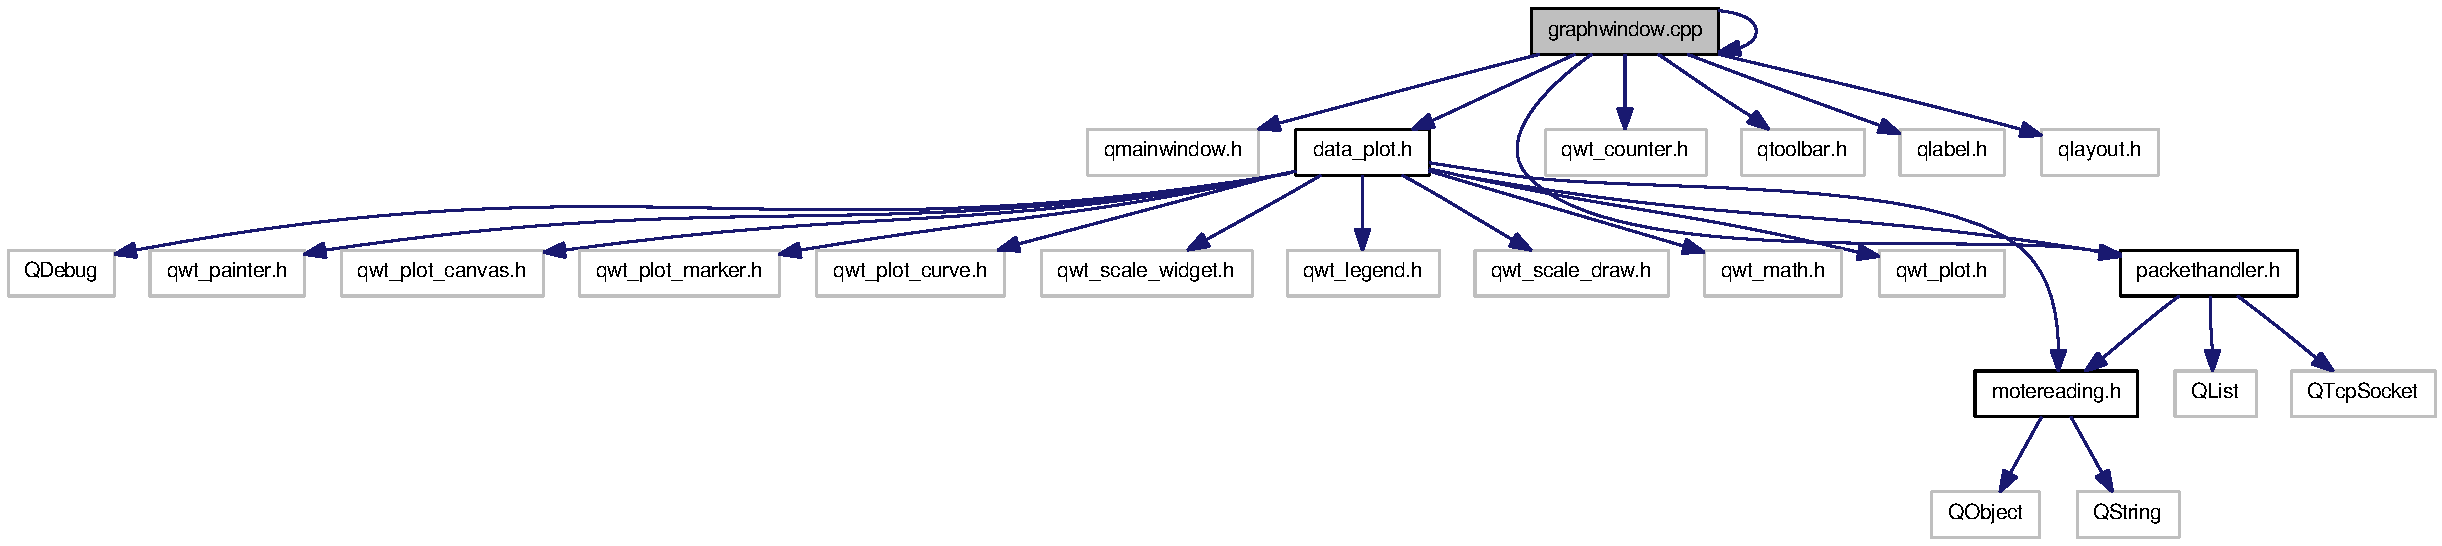
\includegraphics[width=420pt]{graphwindow_8cpp__incl}
\end{center}
\end{figure}
This graph shows which files directly or indirectly include this file:\nopagebreak
\begin{figure}[H]
\begin{center}
\leavevmode
\includegraphics[width=76pt]{graphwindow_8cpp__dep__incl}
\end{center}
\end{figure}


\subsection{Detailed Description}
Implementation of the \hyperlink{classGraphWindow}{GraphWindow} class. \begin{DoxyAuthor}{Author}
Jharrod LaFon 
\end{DoxyAuthor}
\begin{DoxyDate}{Date}
Spring 2010 
\end{DoxyDate}

\hypertarget{graphwindow_8h}{
\section{graphwindow.h File Reference}
\label{graphwindow_8h}\index{graphwindow.h@{graphwindow.h}}
}


Window to display the \hyperlink{classDataPlot}{DataPlot}.  


{\ttfamily \#include $<$qmainwindow.h$>$}\par
{\ttfamily \#include $<$QString$>$}\par
{\ttfamily \#include \char`\"{}data\_\-plot.h\char`\"{}}\par
Include dependency graph for graphwindow.h:\nopagebreak
\begin{figure}[H]
\begin{center}
\leavevmode
\includegraphics[width=420pt]{graphwindow_8h__incl}
\end{center}
\end{figure}
This graph shows which files directly or indirectly include this file:\nopagebreak
\begin{figure}[H]
\begin{center}
\leavevmode
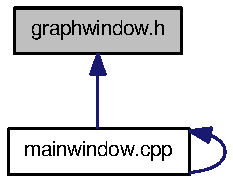
\includegraphics[width=74pt]{graphwindow_8h__dep__incl}
\end{center}
\end{figure}
\subsection*{Classes}
\begin{DoxyCompactItemize}
\item 
class \hyperlink{classGraphWindow}{GraphWindow}
\begin{DoxyCompactList}\small\item\em Window class that contains the \hyperlink{classDataPlot}{DataPlot} widget. \item\end{DoxyCompactList}\end{DoxyCompactItemize}


\subsection{Detailed Description}
Window to display the \hyperlink{classDataPlot}{DataPlot}. Class to display a dataplot widget in a window.

Definition in file \hyperlink{graphwindow_8h_source}{graphwindow.h}.


\hypertarget{main_8cpp}{
\section{main.cpp File Reference}
\label{main_8cpp}\index{main.cpp@{main.cpp}}
}


Main application, entry point.  


{\ttfamily \#include $<$QtGui/QApplication$>$}\par
{\ttfamily \#include \char`\"{}mainwindow.h\char`\"{}}\par
{\ttfamily \#include $<$QMainWindow$>$}\par
{\ttfamily \#include $<$QList$>$}\par
{\ttfamily \#include \char`\"{}packethandler.h\char`\"{}}\par
Include dependency graph for main.cpp:\nopagebreak
\begin{figure}[H]
\begin{center}
\leavevmode
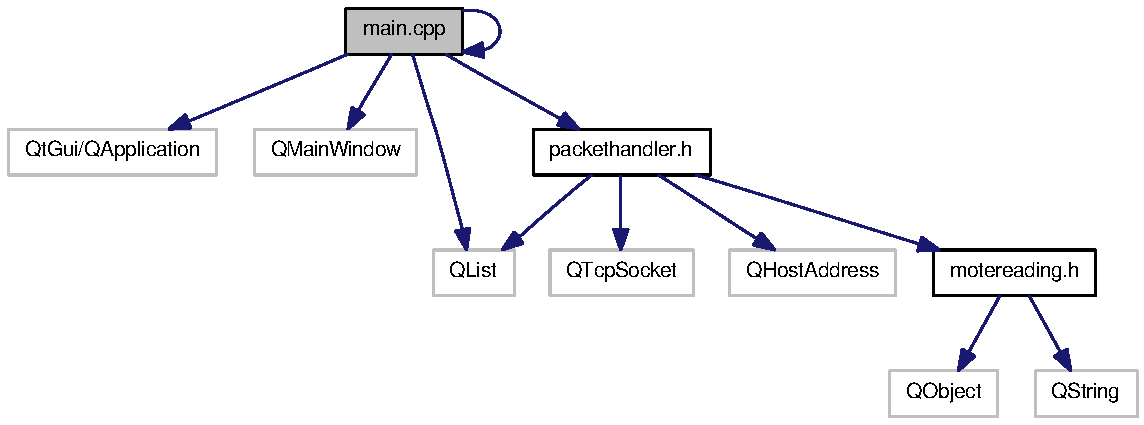
\includegraphics[width=243pt]{main_8cpp__incl}
\end{center}
\end{figure}
This graph shows which files directly or indirectly include this file:\nopagebreak
\begin{figure}[H]
\begin{center}
\leavevmode
\includegraphics[width=59pt]{main_8cpp__dep__incl}
\end{center}
\end{figure}
\subsection*{Functions}
\begin{DoxyCompactItemize}
\item 
\hypertarget{main_8cpp_a0ddf1224851353fc92bfbff6f499fa97}{
int \hyperlink{main_8cpp_a0ddf1224851353fc92bfbff6f499fa97}{main} (int argc, char $\ast$argv\mbox{[}$\,$\mbox{]})}
\label{main_8cpp_a0ddf1224851353fc92bfbff6f499fa97}

\begin{DoxyCompactList}\small\item\em Main function. \item\end{DoxyCompactList}\end{DoxyCompactItemize}


\subsection{Detailed Description}
Main application, entry point. \begin{DoxyAuthor}{Author}
Jharrod LaFon 
\end{DoxyAuthor}
\begin{DoxyDate}{Date}
Spring 2010 
\end{DoxyDate}
\begin{DoxyRemark}{Remarks}
Main application 
\end{DoxyRemark}

\hypertarget{mainwindow_8cpp}{
\section{mainwindow.cpp File Reference}
\label{mainwindow_8cpp}\index{mainwindow.cpp@{mainwindow.cpp}}
}


Implementation of the \hyperlink{classMainWindow}{MainWindow} class.  


{\ttfamily \#include \char`\"{}mainwindow.h\char`\"{}}\par
{\ttfamily \#include \char`\"{}graphwindow.h\char`\"{}}\par
{\ttfamily \#include \char`\"{}ui\_\-mainwindow.h\char`\"{}}\par
{\ttfamily \#include $<$QtCore/QVariant$>$}\par
{\ttfamily \#include $<$QtGui/QAction$>$}\par
{\ttfamily \#include $<$QtGui/QApplication$>$}\par
{\ttfamily \#include $<$QtGui/QButtonGroup$>$}\par
{\ttfamily \#include $<$QtGui/QHeaderView$>$}\par
{\ttfamily \#include $<$QtGui/QLabel$>$}\par
{\ttfamily \#include $<$QtGui/QListWidget$>$}\par
{\ttfamily \#include $<$QtGui/QMainWindow$>$}\par
{\ttfamily \#include $<$QtGui/QMenuBar$>$}\par
{\ttfamily \#include $<$QtGui/QPushButton$>$}\par
{\ttfamily \#include $<$QtGui/QStatusBar$>$}\par
{\ttfamily \#include $<$QtGui/QToolBar$>$}\par
{\ttfamily \#include $<$QtGui/QWidget$>$}\par
Include dependency graph for mainwindow.cpp:\nopagebreak
\begin{figure}[H]
\begin{center}
\leavevmode
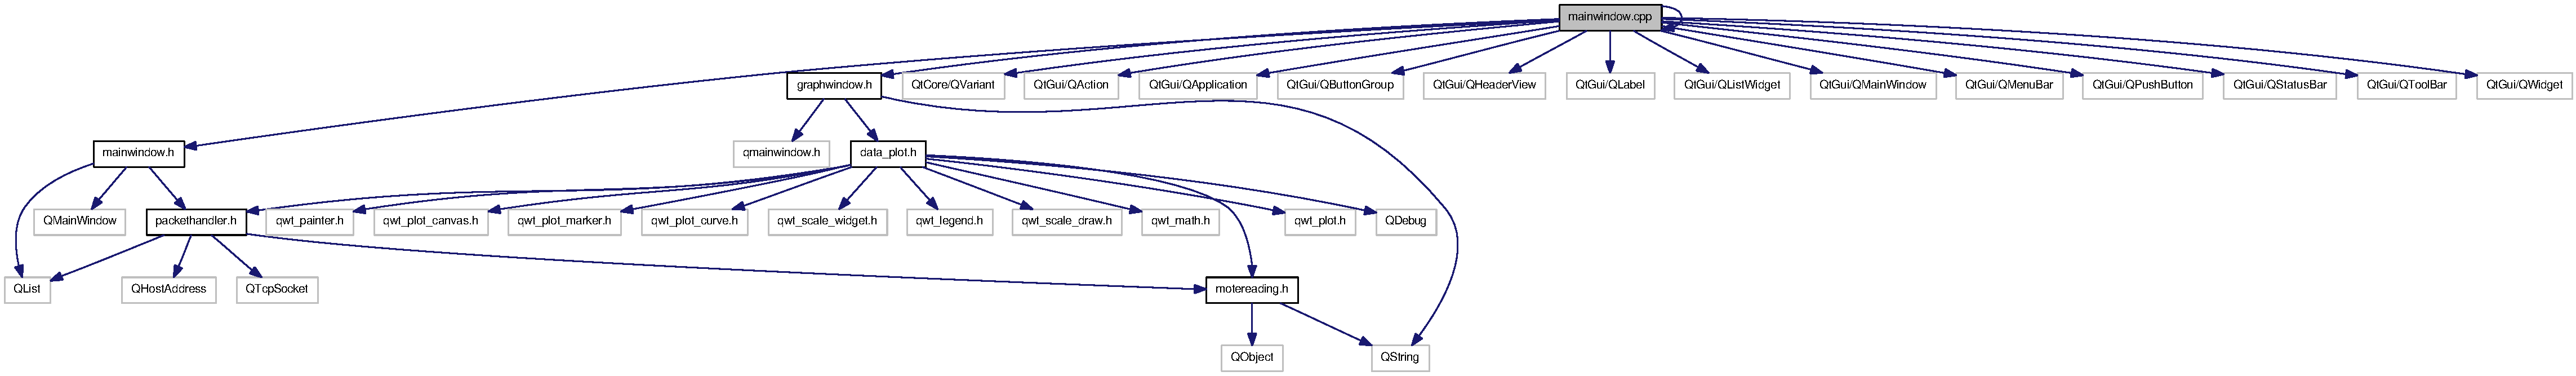
\includegraphics[width=420pt]{mainwindow_8cpp__incl}
\end{center}
\end{figure}
This graph shows which files directly or indirectly include this file:\nopagebreak
\begin{figure}[H]
\begin{center}
\leavevmode
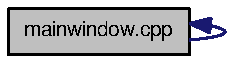
\includegraphics[width=74pt]{mainwindow_8cpp__dep__incl}
\end{center}
\end{figure}


\subsection{Detailed Description}
Implementation of the \hyperlink{classMainWindow}{MainWindow} class. \begin{DoxyAuthor}{Author}
Jharrod LaFon 
\end{DoxyAuthor}
\begin{DoxyDate}{Date}
Spring 2010 
\end{DoxyDate}

\hypertarget{mainwindow_8h}{
\section{mainwindow.h File Reference}
\label{mainwindow_8h}\index{mainwindow.h@{mainwindow.h}}
}


Main Program Window.  


{\ttfamily \#include $<$QMainWindow$>$}\par
{\ttfamily \#include $<$QList$>$}\par
{\ttfamily \#include \char`\"{}packethandler.h\char`\"{}}\par
Include dependency graph for mainwindow.h:\nopagebreak
\begin{figure}[H]
\begin{center}
\leavevmode
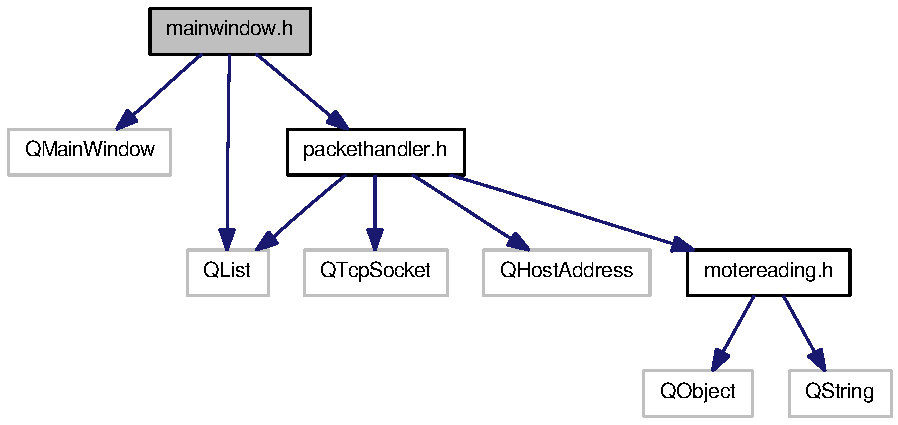
\includegraphics[width=418pt]{mainwindow_8h__incl}
\end{center}
\end{figure}
This graph shows which files directly or indirectly include this file:\nopagebreak
\begin{figure}[H]
\begin{center}
\leavevmode
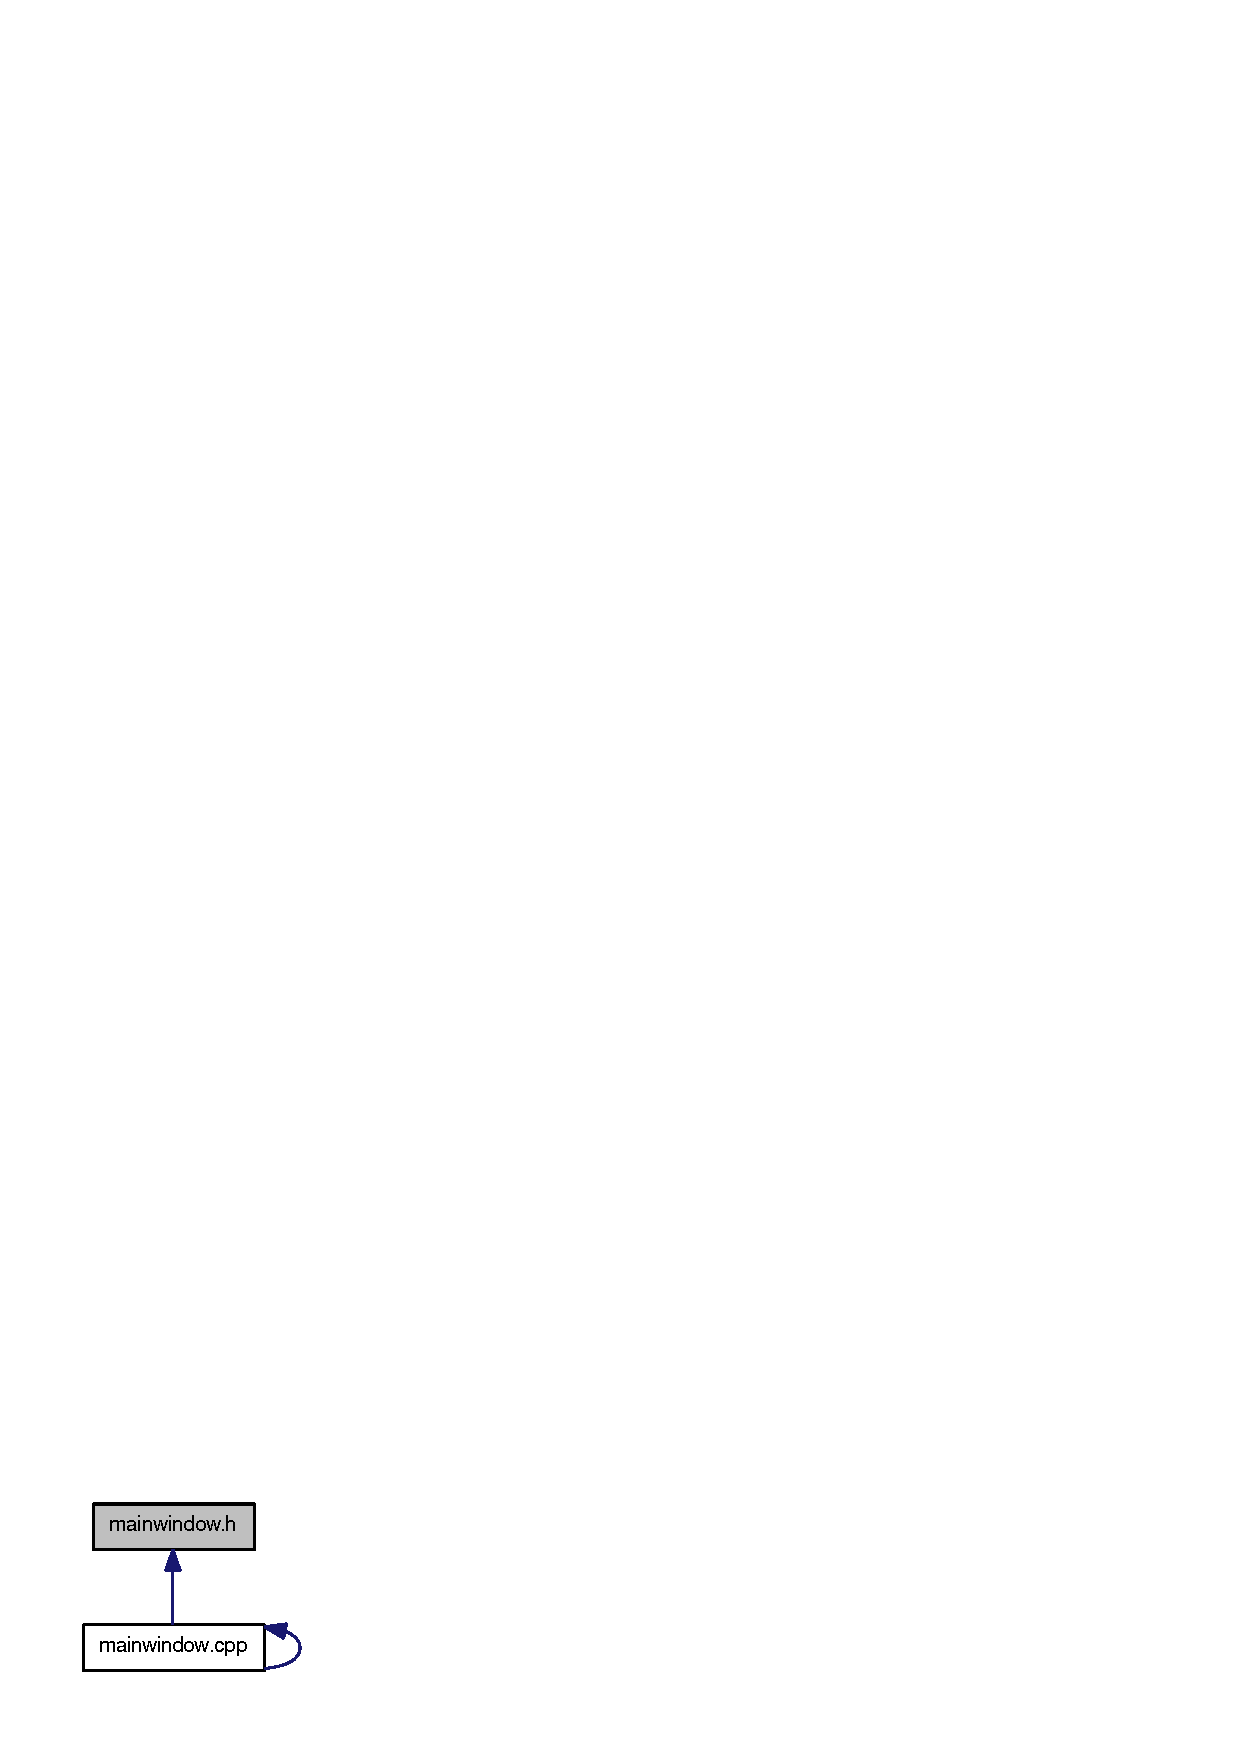
\includegraphics[width=74pt]{mainwindow_8h__dep__incl}
\end{center}
\end{figure}
\subsection*{Classes}
\begin{DoxyCompactItemize}
\item 
class \hyperlink{classMainWindow}{MainWindow}
\begin{DoxyCompactList}\small\item\em The main window class. \item\end{DoxyCompactList}\end{DoxyCompactItemize}


\subsection{Detailed Description}
Main Program Window. 

Definition in file \hyperlink{mainwindow_8h_source}{mainwindow.h}.


\hypertarget{motereading_8cpp}{
\section{motereading.cpp File Reference}
\label{motereading_8cpp}\index{motereading.cpp@{motereading.cpp}}
}


Implementation of the \hyperlink{classMoteReading}{MoteReading} class.  


{\ttfamily \#include \char`\"{}motereading.h\char`\"{}}\par
Include dependency graph for motereading.cpp:\nopagebreak
\begin{figure}[H]
\begin{center}
\leavevmode
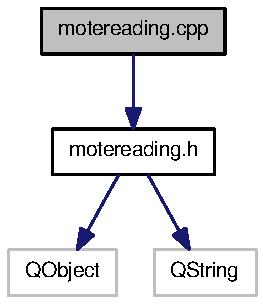
\includegraphics[width=81pt]{motereading_8cpp__incl}
\end{center}
\end{figure}


\subsection{Detailed Description}
Implementation of the \hyperlink{classMoteReading}{MoteReading} class. \begin{DoxyAuthor}{Author}
Jharrod LaFon 
\end{DoxyAuthor}
\begin{DoxyDate}{Date}
Spring 2010 
\end{DoxyDate}

\hypertarget{motereading_8h}{
\section{motereading.h File Reference}
\label{motereading_8h}\index{motereading.h@{motereading.h}}
}


Class to encapsulate sensor readings.  


{\ttfamily \#include $<$QObject$>$}\par
{\ttfamily \#include $<$QString$>$}\par
Include dependency graph for motereading.h:\nopagebreak
\begin{figure}[H]
\begin{center}
\leavevmode
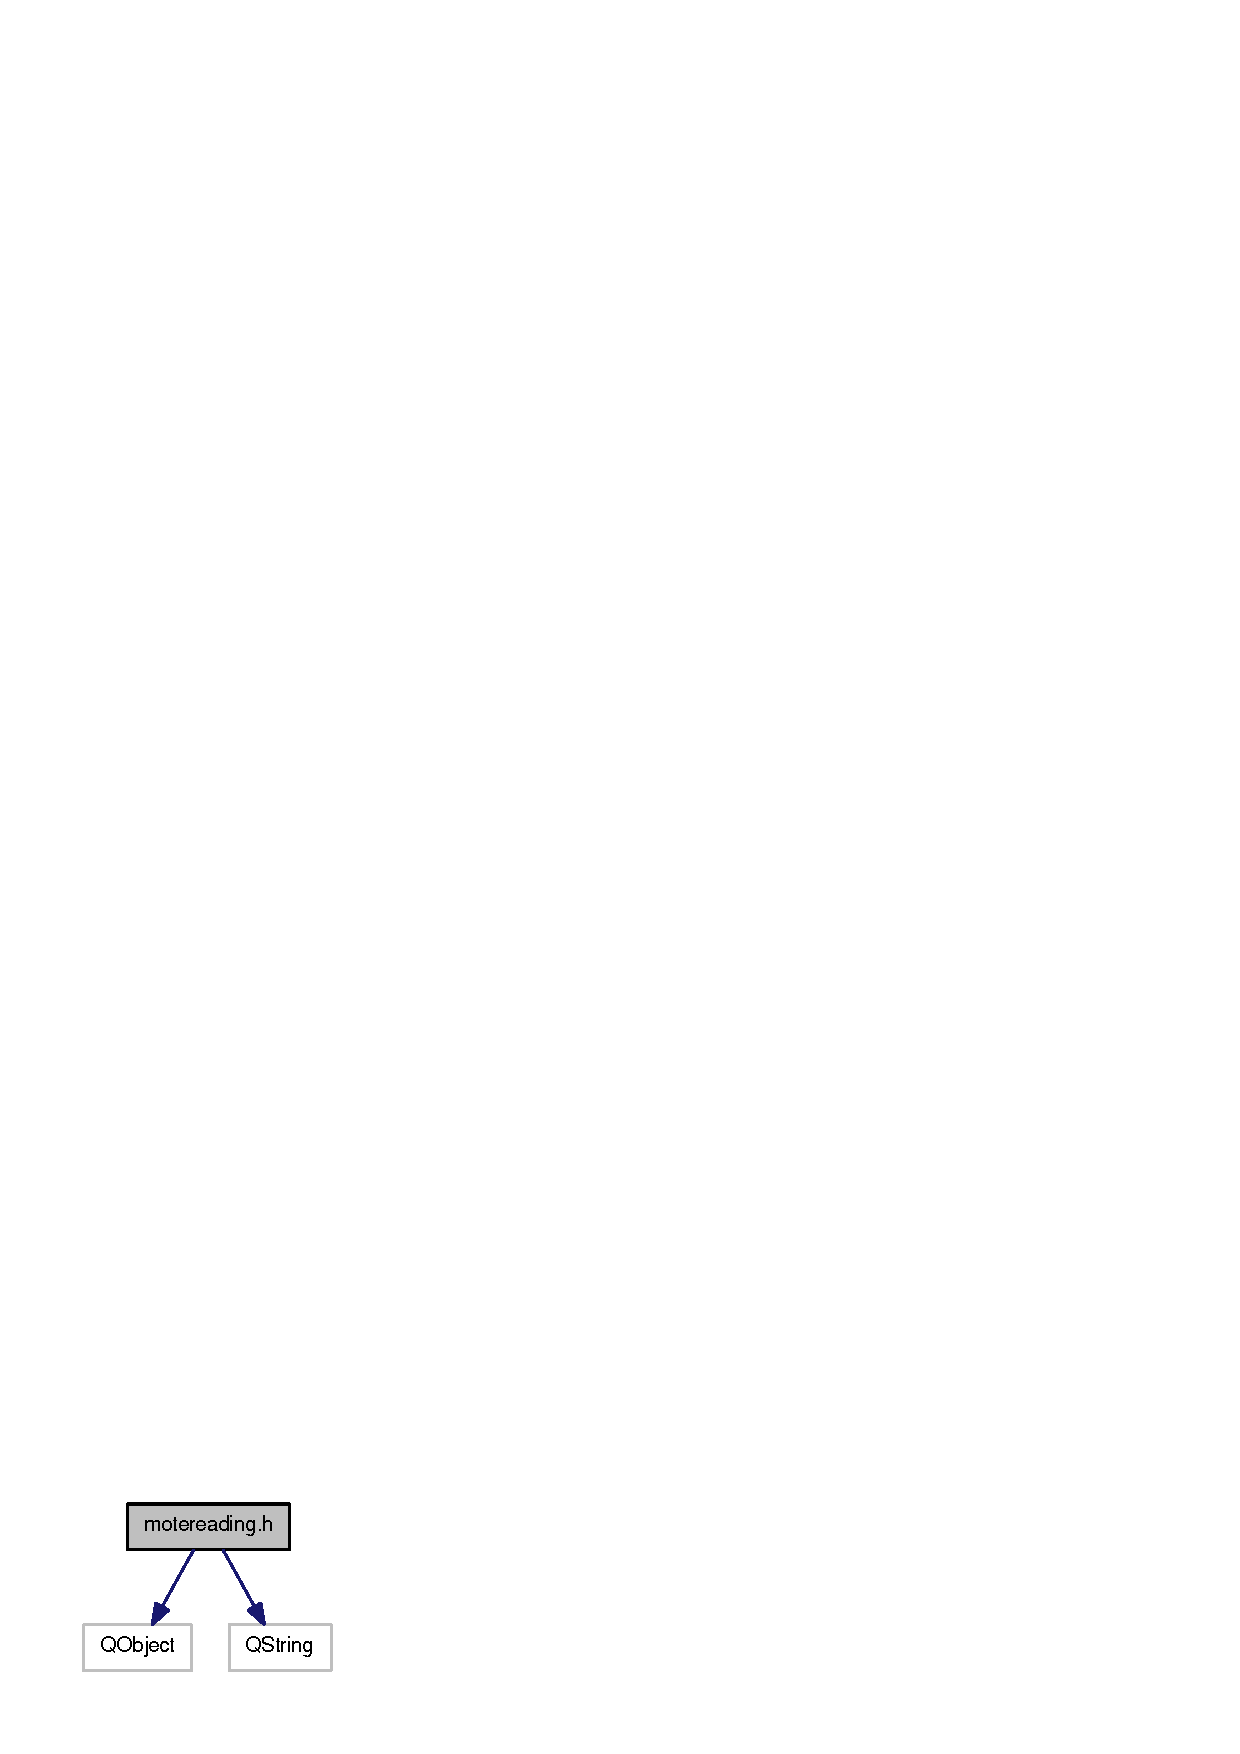
\includegraphics[width=81pt]{motereading_8h__incl}
\end{center}
\end{figure}
This graph shows which files directly or indirectly include this file:\nopagebreak
\begin{figure}[H]
\begin{center}
\leavevmode
\includegraphics[width=250pt]{motereading_8h__dep__incl}
\end{center}
\end{figure}
\subsection*{Classes}
\begin{DoxyCompactItemize}
\item 
class \hyperlink{classMoteReading}{MoteReading}
\begin{DoxyCompactList}\small\item\em Class to encapsulate a sensor reading. \item\end{DoxyCompactList}\end{DoxyCompactItemize}


\subsection{Detailed Description}
Class to encapsulate sensor readings. 
\hypertarget{packethandler_8cpp}{
\section{packethandler.cpp File Reference}
\label{packethandler_8cpp}\index{packethandler.cpp@{packethandler.cpp}}
}


Implementation of \hyperlink{classpacketHandler}{packetHandler} class.  


{\ttfamily \#include \char`\"{}packethandler.h\char`\"{}}\par
{\ttfamily \#include \char`\"{}motereading.h\char`\"{}}\par
{\ttfamily \#include $<$stdint.h$>$}\par
{\ttfamily \#include $<$QDebug$>$}\par
Include dependency graph for packethandler.cpp:\nopagebreak
\begin{figure}[H]
\begin{center}
\leavevmode
\includegraphics[width=418pt]{packethandler_8cpp__incl}
\end{center}
\end{figure}


\subsection{Detailed Description}
Implementation of \hyperlink{classpacketHandler}{packetHandler} class. \begin{DoxyAuthor}{Author}
Jharrod LaFon 
\end{DoxyAuthor}
\begin{DoxyDate}{Date}
Spring 2010 
\end{DoxyDate}


Definition in file \hyperlink{packethandler_8cpp_source}{packethandler.cpp}.


\hypertarget{packethandler_8h}{
\section{packethandler.h File Reference}
\label{packethandler_8h}\index{packethandler.h@{packethandler.h}}
}


Class to serve packets to the \hyperlink{classDataPlot}{DataPlot} class.  


{\ttfamily \#include $<$QTcpSocket$>$}\par
{\ttfamily \#include $<$QHostAddress$>$}\par
{\ttfamily \#include $<$QList$>$}\par
{\ttfamily \#include \char`\"{}motereading.h\char`\"{}}\par
Include dependency graph for packethandler.h:\nopagebreak
\begin{figure}[H]
\begin{center}
\leavevmode
\includegraphics[width=190pt]{packethandler_8h__incl}
\end{center}
\end{figure}
This graph shows which files directly or indirectly include this file:\nopagebreak
\begin{figure}[H]
\begin{center}
\leavevmode
\includegraphics[width=250pt]{packethandler_8h__dep__incl}
\end{center}
\end{figure}
\subsection*{Classes}
\begin{DoxyCompactItemize}
\item 
class \hyperlink{classpacketHandler}{packetHandler}
\begin{DoxyCompactList}\small\item\em Class the serve packets to the \hyperlink{classDataPlot}{DataPlot}. \item\end{DoxyCompactList}\end{DoxyCompactItemize}
\subsection*{Defines}
\begin{DoxyCompactItemize}
\item 
\hypertarget{packethandler_8h_a1d5dab30b404fab91608086105afc78c}{
\#define \hyperlink{packethandler_8h_a1d5dab30b404fab91608086105afc78c}{MAX\_\-BUFFER}~1}
\label{packethandler_8h_a1d5dab30b404fab91608086105afc78c}

\begin{DoxyCompactList}\small\item\em Number of packets to be buffered for each mote. \item\end{DoxyCompactList}\end{DoxyCompactItemize}


\subsection{Detailed Description}
Class to serve packets to the \hyperlink{classDataPlot}{DataPlot} class. 

Definition in file \hyperlink{packethandler_8h_source}{packethandler.h}.


\printindex
\end{document}
